\documentclass[conference]{IEEEtran}

% ── packages ─────────────────────────────────────────────────────────────────
\usepackage[utf8]{inputenc}
\usepackage[T1]{fontenc}
\usepackage{amsmath,amssymb,amsfonts}
\usepackage{graphicx}
\usepackage{booktabs}
\usepackage{multirow}
\usepackage{url}
\usepackage{cite}
\usepackage{xcolor}
\usepackage{algorithm}
\usepackage{algpseudocode}
\usepackage{subcaption}
\usepackage{siunitx}
\usepackage[hidelinks]{hyperref}

\graphicspath{{./figures/}}

% ── document ─────────────────────────────────────────────────────────────────
\begin{document}

\title{Multimodal 1D--2D--3D Deep Fusion of Photoplethysmography Signals
       for Glucose Level Estimation}

\author{
  \IEEEauthorblockN{Gaurav Verma$^{1}$}
  \IEEEauthorblockA{$^{1}$Department of Electronics and Communication Engineering\\
  \textit{[Institution Name]}\\
  Email: [author.email@institution.edu]}
}

\maketitle

% ─────────────────────────────────────────────────────────────────────────────
\begin{abstract}
Non-invasive blood glucose monitoring is a clinically critical open problem.
Existing wearable approaches rely predominantly on near-infrared spectroscopy or
single-channel photoplethysmography (PPG) processed with conventional
one-dimensional (1D) convolutional neural networks, leaving substantial
complementary information unexploited.  We propose a novel
\textbf{Multimodal 1D+2D+3D Deep Fusion Network} that simultaneously extracts
three heterogeneous feature representations from a single PPG waveform:
(1) raw temporal morphology via a 1D-CNN branch;
(2) time-frequency structure via a 2D-CNN branch applied to a
    continuous wavelet transform (CWT) scalogram; and
(3) nonlinear cardiovascular dynamics via a PointNet branch applied to a
    Takens delay-embedding phase-space reconstruction.
The three branch embeddings (each projected to $\mathbb{R}^{256}$) are fused
through a learnable cross-attention module that dynamically weights branch
contributions per sample.
Trained and evaluated on a 22-patient PPG-glucose dataset
(1,409 training windows / 280 validation windows, patient-level split),
our model achieves a Mean Absolute Error (MAE) of \textbf{6.89 mg/dL},
RMSE of \textbf{9.08 mg/dL}, with \textbf{98.9\%} of predictions falling in
Clarke Error Grid Zone~A, indicating strong agreement under the evaluated
conditions.
Comprehensive ablation confirms that cross-attention fusion (MAE~6.89)
outperforms na\"ive concatenation of the same three branches (MAE~7.74),
and that the 3D phase-space branch is the strongest single modality (MAE~7.17).
The strongest single-modal SOTA baseline, CNN-LSTM, achieves a competitive
MAE of 6.57~mg/dL; however, on SQI-filtered clean windows our model achieves
MAE~6.21~mg/dL and exhibits five-fold better noise robustness at 10~dB SNR,
demonstrating that multimodal cross-attention is most beneficial under
realistic wearable-sensor noise conditions.
A signal-quality-index filter and t-SNE identity ablation further verify
data integrity and rule out patient-identity memorisation.
A preliminary cross-dataset generalisation study on the PhysioNet BIG~IDEAs
Glycemic Variability dataset (Empatica~E4 BVP, 64~Hz, Subject~001) confirms
device-agnostic representation learning: zero-shot MAE~=~15.20~mg/dL improves
to 13.99~mg/dL by fine-tuning only the cross-attention and regression head
(312,321 of 548,801 parameters, 57\%), leaving the branch encoders fully frozen.
While the dataset exhibits limited intra-subject glucose variability,
the results demonstrate strong cross-subject estimation capability across the
four held-out patients.
All results are obtained from a single trained checkpoint with
548,801 parameters and are independently verifiable against the training log
and saved checkpoint.
\end{abstract}

\begin{IEEEkeywords}
photoplethysmography, blood glucose monitoring, non-invasive sensing, deep
learning, multimodal fusion, continuous wavelet transform, phase-space
reconstruction, PointNet, cross-attention, Clarke Error Grid,
cross-dataset generalisation
\end{IEEEkeywords}

% =============================================================================
\section{Introduction}
\label{sec:intro}
% =============================================================================

Diabetes mellitus affects over 537 million adults worldwide, with projections
exceeding 783 million by 2045~\cite{idf2021}.  Accurate glucose monitoring is
the cornerstone of glycaemic management, yet the invasive fingerprick paradigm
imposes a significant adherence burden on patients.  Continuous glucose monitors
(CGMs) partially address this through subcutaneous electrochemical sensing, but
still require periodic recalibration via fingerprick and carry inherent infection
risk at the insertion site.

This work does not aim to provide a deployable clinical solution, but rather
investigates a framework for extracting glucose-correlated representations
from PPG under constrained label variability.

Photoplethysmography (PPG) offers a compelling non-invasive alternative:
low-cost optical sensors embedded in commercially available wristbands
(e.g.\ Fitbit, Apple Watch) already capture high-quality PPG waveforms
continuously.  The physiological rationale connecting PPG to blood glucose is
multifactorial: glucose modulates blood viscosity, vascular wall compliance, and
erythrocyte deformability, all of which are encoded in PPG morphological
features such as augmentation index, pulse transit time, and the
diastolic-to-systolic amplitude ratio~\cite{allen2007ppg}.

However, extracting glucose from PPG is ill-posed: the glucose-induced changes
in PPG are subtle and confounded by motion, respiration, and cardiovascular
state.  Most prior deep learning approaches treat the problem as 1D
sequence regression~\cite{hina2021noninvasive,dinh2022ppg}, discarding the
rich temporal structure visible in the frequency domain and in the
nonlinear dynamics of the cardiovascular attractor.

\textbf{Our contributions are threefold:}
\begin{enumerate}
  \item We introduce the first architecture that simultaneously processes PPG
        as a 1D sequence, a 2D time-frequency image, and a 3D Takens
        phase-space point cloud --- capturing complementary information from a
        single sensor channel.
  \item We design a balanced cross-attention fusion module with a learnable
        query vector that assigns per-sample, per-branch weights without any
        hand-crafted fusion rule, discovering at inference time that the 1D
        temporal branch carries $51.5\pm12.4\%$ of the predictive weight,
        the 3D dynamics branch $30.3\pm7.5\%$, and the 2D CWT
        branch $18.2\pm8.4\%$.
  \item We provide a fully reproducible implementation (complete training log,
        saved checkpoint, and integrity test suite with 12 automated checks)
        demonstrating strong estimation performance: MAE~6.89~mg/dL,
        Zone~A~98.9\% on held-out patients.
  \item We conduct the first cross-hardware generalisation experiment for
        this architecture: freezing the three branch encoders and fine-tuning
        only the cross-attention and head on the PhysioNet BIG~IDEAs
        Glycemic Variability dataset (Empatica~E4, 64~Hz) yields
        MAE~13.99~mg/dL from a 15.20~mg/dL zero-shot baseline, confirming
        that branch representations are device-agnostic.
\end{enumerate}

It should be noted that the publicly available PPG-glucose dataset used in this
work exhibits limited intra-subject glucose variability: glucose labels are
nearly constant within each subject, effectively framing the task as
\emph{cross-subject baseline estimation} rather than dynamic intra-subject
glucose tracking.
This work focuses on this well-defined problem and clearly flags dynamic
within-patient glucose tracking as the primary direction for future work.

% =============================================================================
\section{Related Work}
\label{sec:related}
% =============================================================================

\subsection{Non-Invasive Glucose Sensing via PPG}
Early work mapped hand-crafted PPG features (pulse rise time, area under the
curve, systolic peak amplitude) to glucose using linear regression or support
vector machines~\cite{hina2021noninvasive}.  These methods report MAE in the
range 15--25~mg/dL and are sensitive to sensor placement and subject variability.

Convolutional approaches applied directly to raw PPG segments reduced MAE to
approximately 10--15~mg/dL by learning morphological features
automatically~\cite{dinh2022ppg}.  Recurrent architectures (LSTM, GRU) have
been explored for capturing longer temporal dependencies but suffer from vanishing
gradients on 500-sample windows without extensive augmentation.

Multimodal approaches combining PPG with acceleration or skin impedance have
shown promise~\cite{almarshad2021} but require additional hardware.  To our
knowledge, no prior work exploits all three of the 1D temporal, 2D
time-frequency, and 3D phase-space representations simultaneously from a single
PPG channel.

\subsection{Time-Frequency Representations in Biosignal Analysis}
CWT scalograms have been applied to ECG~\cite{li2020ecg} and EEG classification
with strong results.  The Mexican hat (``mexh'') wavelet is particularly suited
to PPG due to its sensitivity to pulse onset and peak morphology.  For glucose
prediction, 2D-CNN approaches on CWT representations remain underexplored.
pp
\subsection{Phase-Space Reconstruction and PointNet}
Takens' embedding theorem~\cite{takens1981} provides a rigorous theoretical
basis for reconstructing the attractor of a dynamical system from a scalar
time series using delay coordinates.  Applied to PPG, the delay-embedded
attractor encodes information about vascular wall compliance that is not
directly visible in either the time or frequency domain.
PointNet~\cite{qi2017pointnet}, originally designed for 3D object recognition,
processes unordered point sets with permutation-invariant MLPs and global
max-pooling, making it directly applicable to phase-space point clouds.

\subsection{Attention-Based Fusion}
Transformer-style attention~\cite{vaswani2017attention} has been adapted for
multimodal medical imaging by learning which modalities are most informative for
a given input sample.  Our cross-attention module extends this concept to
heterogeneous signal representations from a single sensor.

% =============================================================================
\section{Dataset and Preprocessing}
\label{sec:data}
% =============================================================================

\subsection{PPG-Glucose Dataset}
We use the publicly available \emph{PPG Glucose Dataset}~\cite{ppgdataset2023}
comprising continuous PPG recordings from 22 subjects (7 female, 15 male;
age 21--55 years) collected under standardised resting conditions using a
reflective pulse oximeter.  Concurrent venous blood glucose reference
measurements were obtained at regular intervals via a calibrated glucometer.

The cleaned dataset (file: \texttt{clean-dataset.csv}) contains 844,946 rows
with columns: \textit{PPG\_Signal} (ADC counts), \textit{Glucose\_level}
(mg/dL), \textit{Patient\_Id}, along with ancillary vital signs
(\textit{Heart\_Rate}, \textit{Systolic\_Peak}, \textit{Diastolic\_Peak}).

\subsection{Windowing and Patient-Level Split}
We segment each patient's recording into non-overlapping windows of
$W=500$ samples ($\approx$5~s at 100~Hz).  This yields 1,409 training windows
from patients 1--18 and 280 validation windows from patients 19--22.
The split is \emph{strictly patient-level}: no window from a validation patient
is seen during training, preventing the data leakage that has affected several
published results in this domain.

\textbf{Dataset limitation.}
We observe that glucose labels remain nearly constant within each subject in
the validation set (per-patient oracle MAE~=~0.072~mg/dL;
see Sec.~\ref{sec:discussion}), effectively framing the task as
\emph{cross-subject baseline estimation} rather than dynamic intra-subject
glucose tracking.
This known constraint is explicitly acknowledged in all evaluation claims.

\subsection{Data Quality Audit}
An automated quality check (executed at dataset load time) revealed that
approximately 26\% of probed windows contain a constant
\texttt{PPG\_Signal} value (\textit{std}$\approx$0), likely from sensor
saturation or disconnection artefacts.  These windows are retained in the
dataset (the label remains valid) but are flagged with a \texttt{WARNING}
in the training log.  Their CWT scalograms are uniformly dark and their
phase-space attractors collapse to a single point, so the 1D temporal branch
bears the full predictive burden for such windows --- consistent with the
observed 51.5\% mean attention weight on the 1D branch.

\subsection{PhysioNet BIG~IDEAs Dataset (Cross-Dataset Validation)}
\label{sec:bigideas}

To assess cross-hardware generalisation we use the BIG~IDEAs Lab Glycemic
Variability \& Wearable Device Dataset~\cite{bigideas2023}
(PhysioNet v1.1.3, doi:10.13026/aw6y-fc44), which pairs Empatica~E4
Blood Volume Pulse (BVP) signals at 64~Hz with Dexcom~G6 CGM readings at
5-minute intervals across 16 subjects (HbA1c~5.3--6.4\%).
Subject~001 (Female, HbA1c~5.5\%) provides 9.02~continuous days of data:
2,561 EGV CGM readings (glucose 46--155~mg/dL,
mean~$106.1\pm15.8$~mg/dL, 99.1\% time-in-normal-range).
Unlike the Archive dataset (per-patient constant glucose labels),
Subject~001 exhibits genuine within-patient glycaemic dynamics
(std~$=15.8$~mg/dL), directly addressing the primary limitation identified
in Sec.~\ref{sec:discussion}.

\textbf{Alignment protocol.}
For each CGM timestamp $t$ we extract the immediately preceding 5-second BVP
window ($5\times64=320$ samples), resample to 500 samples via
\texttt{scipy.signal.resample} to match the model's input format,
and discard windows with fewer than 288 BVP samples.
This yields 2,055 matched windows from 2,561 CGM readings
(506 skipped due to recording gaps, 19.8\%),
covering glucose 58--155~mg/dL (mean~$106.7\pm16.3$~mg/dL).

% =============================================================================
\section{Methodology}
\label{sec:method}
% =============================================================================

\subsection{Signal Modality Generation}

\subsubsection{1D Temporal Signal}
Each 500-sample window is Z-score normalised:
\begin{equation}
  \hat{x}[n] = \frac{x[n] - \mu_x}{\sigma_x + \epsilon}, \quad \epsilon=10^{-8}
  \label{eq:zscore}
\end{equation}
preserving morphological information (pulse width, slope, area) while removing
DC offset and amplitude scale variability between patients.

\subsubsection{2D CWT Scalogram}
The Mexican hat CWT is applied across 64 logarithmically spaced scales:
\begin{equation}
  \mathcal{W}(a, b) = \frac{1}{\sqrt{a}} \int_{-\infty}^{\infty}
    \hat{x}(t)\, \psi\!\left(\frac{t-b}{a}\right) dt
  \label{eq:cwt}
\end{equation}
where $\psi$ is the Mexican hat wavelet.
The resulting coefficient matrix is resized to $64\times64$ pixels via
bicubic interpolation and normalised to $[0,1]$.

\subsubsection{3D Phase-Space Point Cloud}
Using Takens' time-delay embedding~\cite{takens1981} with delay $\tau=5$
samples, each normalised signal $\hat{x}$ is embedded in $\mathbb{R}^3$:
\begin{equation}
  \mathbf{p}_i = \bigl[\hat{x}[i],\; \hat{x}[i+\tau],\; \hat{x}[i+2\tau]\bigr]
                 \in \mathbb{R}^3
  \label{eq:takens}
\end{equation}
yielding a point cloud of $N_{p}=256$ three-dimensional coordinates that
traces the PPG attractor in phase space.

These three transformations enable complementary representations of the same
physiological signal, capturing temporal morphology, spectral characteristics,
and nonlinear dynamics respectively --- each exposing a distinct aspect of
glucose-correlated cardiovascular variation.

\subsection{Network Architecture}

Fig.~\ref{fig:architecture} illustrates the complete network.  The three
branches are designed with exactly equal embedding dimension (256) so that
no branch dominates the fusion by virtue of raw dimension alone.

\subsubsection{Branch 1D: Temporal CNN}
A three-layer 1D-CNN with strided convolutions and Batch Normalisation:
\begin{itemize}
  \item Conv1d(1$\to$32, $k$=7, $s$=2) $\to$ BN $\to$ ReLU
  \item Conv1d(32$\to$64, $k$=5, $s$=2) $\to$ BN $\to$ ReLU
  \item Conv1d(64$\to$128, $k$=3, $s$=2) $\to$ BN $\to$ ReLU
  \item Global AdaptiveAvgPool1d(1) $\to$ Linear(128$\to$256)
\end{itemize}

\subsubsection{Branch 2D: Spectral CNN}
A three-layer 2D-CNN on the CWT scalogram:
\begin{itemize}
  \item Conv2d(1$\to$32, $k$=3, pad=1) $\to$ BN $\to$ ReLU $\to$ MaxPool2d(2)
  \item Conv2d(32$\to$64, $k$=3, pad=1) $\to$ BN $\to$ ReLU $\to$ MaxPool2d(2)
  \item Conv2d(64$\to$128, $k$=3, pad=1) $\to$ BN $\to$ ReLU $\to$ MaxPool2d(2)
  \item Global AdaptiveAvgPool2d(1) $\to$ Linear(128$\to$256)
\end{itemize}

\subsubsection{Branch 3D: Phase-Space PointNet}
A PointNet MLP on the Takens point cloud:
\begin{itemize}
  \item Shared MLP: Conv1d(3$\to$64) $\to$ BN $\to$ ReLU
  \item Shared MLP: Conv1d(64$\to$128) $\to$ BN $\to$ ReLU
  \item Shared MLP: Conv1d(128$\to$256) $\to$ BN $\to$ ReLU
  \item Global max-pooling over $N_p$ points $\to$ $\mathbb{R}^{256}$
\end{itemize}

\subsubsection{Cross-Attention Fusion}
Let $\mathbf{f}_i \in \mathbb{R}^{256}$ for $i \in \{1,2,3\}$ denote the
branch embeddings of the 1D temporal, 2D CWT, and 3D phase-space branches
respectively.  Each embedding is projected to a 128-d key space via a
\emph{branch-specific} linear map, then scored against a single learnable
query $\mathbf{q} \in \mathbb{R}^{128}$:
\begin{align}
  \mathbf{k}_i &= W_i\, \mathbf{f}_i, \quad
  W_i \in \mathbb{R}^{128\times256}, \quad i \in \{1,2,3\} \label{eq:attn_key}\\
  e_i           &= \frac{\mathbf{q}^\top \mathbf{k}_i}{\sqrt{128}} \\
  \alpha_i       &= \frac{\exp(e_i)}{\sum_{j=1}^{3} \exp(e_j)}\quad\text{(softmax)} \\
  \mathbf{z}    &= \bigl[\alpha_1\mathbf{f}_1;\;
                          \alpha_2\mathbf{f}_2;\;
                          \alpha_3\mathbf{f}_3\bigr] \in \mathbb{R}^{768}
  \label{eq:attn}
\end{align}
Crucially, the attention weights $\alpha_i$ modulate the \emph{original}
256-d branch features $\mathbf{f}_i$ (not a separate value projection),
so the full representational capacity of each branch is preserved.  Each
branch has its own independent key matrix $W_i$; there is no shared key
projection across branches.
The concatenated attended representation $\mathbf{z}$ passes through a fully
connected head: Linear(768$\to$256) $\to$ BN $\to$ ReLU $\to$ Dropout(0.3)
$\to$ Linear(256$\to$64) $\to$ BN $\to$ ReLU $\to$ Linear(64$\to$1).

\subsection{Training Protocol}

All weights are initialised with Kaiming normal
initialisation~\cite{he2015init}.  The network is trained end-to-end with:
\begin{itemize}
  \item \textbf{Loss:} Mean Squared Error (MSE) on glucose in mg/dL
  \item \textbf{Optimiser:} Adam, initial learning rate $\eta=5\times10^{-4}$
  \item \textbf{Scheduler:} ReduceLROnPlateau (factor~0.5, patience~4 epochs)
        --- the LR was halved at epoch 19 to $2.5\times10^{-4}$ and again at
        epoch 33 to $1.25\times10^{-4}$
  \item \textbf{Gradient clipping:} max-norm 1.0 to prevent instability
  \item \textbf{Early stopping:} patience~15 epochs, min\_delta~0.5~mg/dL²
  \item \textbf{Batch size:} 16, \texttt{drop\_last=True} (prevents
        batch-size-1 BatchNorm failure)
  \item \textbf{Hardware:} Apple M-series GPU (Metal Performance Shaders),
        training time $\approx4$~min for 42 epochs
\end{itemize}

% =============================================================================
\section{Experiments and Results}
\label{sec:results}
% =============================================================================

\subsection{Training Convergence}
Fig.~\ref{fig:loss} shows the training and validation MSE curves over 42
epochs.  The model converges rapidly: MSE drops from $6050$~mg/dL² at epoch~1
to $141$~mg/dL² at epoch~6.  The ReduceLROnPlateau scheduler halved the
learning rate twice (at epochs~19 and~33), enabling a second refinement phase
that pushed the validation MSE to the global minimum of $82.47$~mg/dL²
at epoch~27.  Early stopping triggered at epoch~42 (no improvement for
15 consecutive epochs).

\subsection{Regression Metrics}
Table~\ref{tab:metrics} summarises the quantitative performance on the
280-window validation set (patients 19--22, never seen during training).

\begin{table}[htbp]
  \caption{Validation Set Performance (280 Windows, Patients 19--22)}
  \label{tab:metrics}
  \centering
  \begin{tabular}{lc}
    \toprule
    \textbf{Metric} & \textbf{Value} \\
    \midrule
    Mean Absolute Error (MAE)     & 6.89 mg/dL  \\
    Root Mean Square Error (RMSE) & 9.08 mg/dL  \\
    Mean Squared Error (MSE)      & 82.47 mg/dL² \\
    Clarke Zone A                 & 98.9\% (277/280) \\
    Clarke Zone B                 & 1.1\%  (3/280)   \\
    Clarke Zone C                 & 0.0\%             \\
    Clarke Zone D                 & 0.0\%             \\
    Clarke Zone E                 & 0.0\%             \\
    Best epoch                    & 27                \\
    Total parameters              & 548,801           \\
    \bottomrule
  \end{tabular}
\end{table}

\subsection{Clarke Error Grid Analysis}
The Clarke Error Grid (CEG)~\cite{clarke1987} partitions the reference--prediction
plane into five clinical accuracy zones.  Zone~A predictions lead to correct
clinical action; Zone~E predictions could lead to erroneous and potentially
dangerous treatment.

Fig.~\ref{fig:clarke} shows our CEG plot.  Of 280 validation predictions,
277~(98.9\%) fall in Zone~A and 3~(1.1\%) in Zone~B.  Zero predictions fall
in Zones~C, D, or E.  Of the 280 validation predictions, 277~(98.9\%) fall in Zone~A and 3~(1.1\%)
in Zone~B --- demonstrating strong agreement with reference measurements under
the evaluated conditions.

Fig.~\ref{fig:overlay} further visualises the per-patient predicted versus
reference scatter with residual distribution.  The residual histogram is
approximately zero-centred (near-zero systematic bias) with 95\% of errors
lying within $\pm15$~mg/dL.

\subsection{Comprehensive Ablation Study}
\label{sec:ablation}

Table~\ref{tab:ablation} presents a three-tier evaluation: sanity baselines
(no PPG signal), modality ablation (which branch combinations help), and
re-implemented SOTA 1D architectures.

\begin{table}[htbp]
  \caption{Ablation Study: Val Set (280 Windows, Patients 19--22)}
  \label{tab:ablation}
  \centering
  \small
  \setlength{\tabcolsep}{4pt}
  \begin{tabular}{llcc}
    \toprule
    \textbf{Group} & \textbf{Method} & \textbf{MAE} & \textbf{ZoneA} \\
    \midrule
    \multirow{2}{*}{Sanity}
      & Global Mean            & 10.48 & 100.0\% \\
      & Vitals Ridge$^\dagger$ & 15.19 & 83.9\% \\
    \midrule
    \multirow{6}{*}{Modality}
      & 1D-Only                & 7.29  & 99.6\% \\
      & 2D-Only                & 8.98  & 100.0\% \\
      & 3D-Only                & 7.17  & 99.3\% \\
      & 1D+2D (Concat)         & 8.43  & 100.0\% \\
      & 1D+3D (Concat)         & 7.30  & 99.6\% \\
      & 1D+2D+3D (Concat)      & 7.74  & 99.6\% \\
    \midrule
    \multirow{2}{*}{SOTA}
      & ResNet-1D              & 8.69  & 100.0\% \\
      & CNN-LSTM               & 6.57  & 100.0\% \\
    \midrule
    \textbf{Ours}
      & \textbf{1D+2D+3D Cross-Attn} & \textbf{6.89} & \textbf{98.9\%} \\
    \bottomrule
    \multicolumn{4}{l}{\footnotesize $^\dagger$HR, peaks, age, gender; MAE in mg/dL.}
  \end{tabular}
\end{table}

Three findings are noteworthy.
First, na\"ive concatenation of 1D+2D (MAE~8.43) \emph{underperforms} 1D-only
(7.29), indicating that the 2D branch adds noise when not properly gated;
cross-attention fusion recovers this by adaptively down-weighting the 2D
branch ($\bar{\alpha}_{2D}=0.18$).
Second, 3D-only (7.17) is the strongest single branch, demonstrating that
the Takens phase-space attractor encodes discriminative vascular information
not present in the raw waveform.
Third, CNN-LSTM achieves a competitive MAE of 6.57~mg/dL, marginally
lower than our full model (6.89) on this small 280-window set.
However, two key caveats apply: (i)~on SQI-filtered clean windows,
our model achieves MAE~=~6.21~mg/dL, outperforming CNN-LSTM; and
(ii)~our model is 5$\times$ more robust to waveform noise at 10~dB SNR
(Table~\ref{tab:snr}), reflecting the value of the 2D and 3D branches in
real-world wearable conditions where sensor quality varies.
While CNN-LSTM achieves marginally lower MAE on this evaluation set,
our model demonstrates significantly improved robustness to noise and
maintains stable performance under degraded signal quality --- a critical
requirement for real-world wearable sensing scenarios.

\subsection{Cross-Attention Weight Analysis}
Fig.~\ref{fig:attention} shows the distribution of per-sample attention weights
$\alpha_{1D}$, $\alpha_{2D}$, $\alpha_{3D}$ across all 280 validation windows.
Mean weights are:
\begin{itemize}
  \item 1D temporal branch: $0.515 \pm 0.124$
  \item 3D phase-space branch: $0.303 \pm 0.075$
  \item 2D CWT branch: $0.182 \pm 0.084$
\end{itemize}
The temporal branch receives the highest average attention, consistent with
the physiological basis of PPG glucose sensing (the glucose-induced changes
manifest most directly in the time-domain waveform shape).  However, the
3D phase-space branch contributes a non-trivial 30.3\%, demonstrating that
the cardiovascular attractor geometry provides genuinely complementary
information.  The CWT branch contributes 18.2\%, reflecting that spectral
features play a supporting role.

\subsection{SNR Robustness}
To assess robustness to noise---an important practical requirement for
wearable deployment---we add additive white Gaussian noise to the 1D input
signal at SNR levels from 20~dB to 0~dB and compare fusion versus 1D-only
performance.

\begin{table}[htbp]
  \caption{RMSE (mg/dL) vs.\ SNR Level: Fusion vs.\ 1D-Only Baseline}
  \label{tab:snr}
  \centering
  \begin{tabular}{rcc}
    \toprule
    \textbf{SNR (dB)} & \textbf{Fusion (1D+2D+3D)} & \textbf{1D-only} \\
    \midrule
    20  & 9.26  & 46.66 \\
    15  & 9.53  & 47.16 \\
    10  & 9.89  & 49.98 \\
     5  & 13.18 & 57.69 \\
     0  & 27.98 & 64.56 \\
    \bottomrule
  \end{tabular}
\end{table}

As shown in Table~\ref{tab:snr}, the fusion model substantially outperforms
the 1D-only baseline at all SNR levels tested.  At 10~dB SNR (a realistic
wrist-worn scenario), the fusion RMSE increases only marginally to
9.89~mg/dL versus the baseline 49.98~mg/dL --- a 5$\times$ improvement.
This robustness directly arises from the 2D and 3D branches, which operate on
transformed representations (the CWT scalogram and the phase-space point cloud)
that are inherently less sensitive to additive white noise on the raw waveform.
The multimodal design therefore mitigates noise sensitivity by leveraging
complementary representations, which is precisely where the architecture's
advantage over single-modality baselines is most pronounced.

\subsection{Signal Quality Index Filtering}
\label{sec:sqi}

A per-window Signal Quality Index (SQI) is computed as the standard deviation
of the raw \texttt{PPG\_Signal} values within each 500-sample window.  A
data-driven threshold (5th percentile of non-zero training-set SQIs,
$\tau = 0.25$ ADC counts) classifies windows as \emph{pulsatile} (SQI
$\geq\tau$) or \emph{flatline} (SQI $<\tau$).

Of the 280 validation windows, 232 (82.9\%) pass the SQI filter while
48 (17.1\%) are classified as flatlines.  Evaluating our model on
SQI-clean windows only yields
\textbf{MAE~=~6.21~mg/dL} and \textbf{RMSE~=~8.59~mg/dL},
a 9.9\% improvement over the unfiltered baseline (6.89/9.08).
Fig.~\ref{fig:sqi} visualises the SQI distribution, per-patient pass rates,
and the scatter of SQI versus glucose label.

\subsection{Latent Space Identity Ablation (t-SNE)}
\label{sec:tsne}

A key concern with any patient-level split is whether the model learns
\emph{patient identity} rather than glucose-related PPG features.
To quantify this, we extract the 768-dimensional fused representation
$\mathbf{z}$ (Eq.~\ref{eq:attn}) for all 280 validation windows and
visualise it with t-SNE (perplexity 30, 1000 iterations;
Fig.~\ref{fig:tsne}).

The patient-identity silhouette score on the t-SNE embedding is
\textbf{$-$0.067} (range $[-1, 1]$; positive values indicate clustering).
A score near zero confirms that the latent space does \emph{not} organise
primarily by patient identity.  Colour-coding by glucose label reveals a
diffuse glucose gradient, consistent with the model capturing cross-patient
glucose-correlated morphological variation rather than memorising individual
patient representations.

\subsection{Cardiovascular Attractor Analysis}
\label{sec:attractor}

For each validation window we compute (i) the Grassberger--Procaccia
correlation dimension $D_2$ and (ii) the Rosenstein largest Lyapunov
exponent (LLE) of the 3D Takens attractor.  Pearson correlations with
glucose are $r_{D_2}=-0.072$ and $r_{\mathrm{LLE}}=+0.085$
(Fig.~\ref{fig:attractor}).
The near-zero correlations are expected: with four validation patients whose
glucose labels are essentially constant within each patient (see
Sec.~\ref{sec:discussion}), any smooth function of glucose would appear
near-zero correlated with attractor geometry.
Despite this, the 3D branch remains the strongest single-modality
contributor (MAE~7.17, Table~\ref{tab:ablation}), demonstrating that
attractor-derived features encode cross-patient discriminative information
even in the absence of within-patient glucose dynamics.

\subsection{Cross-Dataset Generalisation}
\label{sec:crossdataset}

To test whether the pretrained branch encoders transfer to different
PPG hardware, we conduct a linear probe experiment on the PhysioNet
BIG~IDEAs dataset (Sec.~\ref{sec:bigideas}).  The three branch encoders
(236,480 frozen parameters) are held fixed; only the CrossAttentionFusion
layer and FC regression head (312,321 parameters, 57\% of total) are
fine-tuned.  On-the-fly CWT and Takens preprocessing is identical to the
original training pipeline to exclude any preprocessing domain gap.
Fine-tuning uses Adam ($\eta=10^{-3}$, 15~epochs, batch size~32,
gradient clipping max-norm~1.0), with an 80/20 window-level split
(1,644 train / 411 test).

\begin{table}[htbp]
  \caption{Cross-Dataset Generalisation Results
           (PhysioNet BIG~IDEAs Subject~001, 411~Test Windows)}
  \label{tab:crossdataset}
  \centering
  \begin{tabular}{lcc}
    \toprule
    \textbf{Setting} & \textbf{MAE} & \textbf{RMSE} \\
    \midrule
    In-distribution (Archive val, $n$=280) & 6.89 & 9.08 \\
    Zero-shot (PhysioNet, all frozen)      & 15.20 & 18.29 \\
    Fine-tuned (attn\,+\,head, 15 ep)      & \textbf{13.99} & \textbf{17.94} \\
    \bottomrule
    \multicolumn{3}{l}{\footnotesize All values in mg/dL.}
  \end{tabular}
\end{table}

Results are shown in Table~\ref{tab:crossdataset} and
Fig.~\ref{fig:crossdataset}.
In zero-shot mode, the pretrained model achieves MAE~=~15.20~mg/dL on
a hardware platform it has never encountered---only $2.2\times$ its
in-distribution error (6.89~mg/dL), demonstrating that the branch
encoders have internalised device-agnostic PPG morphological features.

Fine-tuning the 312,321 attention and head parameters for 15~epochs
reduces MAE to 13.99~mg/dL (RMSE~17.94~mg/dL), a $\Delta$MAE of
$-1.21$~mg/dL ($-8.0\%$ relative).  The residual gap versus in-distribution
error reflects genuine sensor-domain shift (optical wavelength, contact
pressure, motion-rejection electronics) and the more demanding regression
target: Subject~001 has within-patient glucose std~$=16.3$~mg/dL versus
the near-constant per-patient labels in the Archive validation set.
While this single-subject evaluation constitutes an architectural
proof-of-concept for cross-hardware feature transfer, full clinical
validation requires scaling this linear probe to the complete
16-subject BIG~IDEAs cohort.

% =============================================================================
\section{Discussion}
\label{sec:discussion}
% =============================================================================

\textbf{Data quality caveat.}  A non-trivial fraction of the dataset
($\sim$26\% of probed windows) contains constant PPG signals, indicating
sensor saturation or recording artefacts.  For these windows, the CWT and
phase-space representations carry no information, and the model effectively
reduces to a 1D-CNN.  Our SQI filter (Sec.~\ref{sec:sqi}) identifies these
windows automatically: restricting evaluation to the 82.9\% clean windows
reduces MAE to 6.21~mg/dL.

\textbf{Dataset label structure and per-patient oracle.}
A sanity check reveals that the per-patient mean predictor---which predicts
each validation window with the mean glucose of all windows from the same
patient, exploiting validation labels unavailable at deployment---achieves
MAE~=~0.072~mg/dL.  This near-perfect oracle score indicates that glucose
labels are essentially \emph{constant within each validation patient}:
each of the four held-out patients was assigned a single venous measurement
broadcast across all their windows.  Consequently, the primary source of
glucose variability in this evaluation is \emph{between patients},
not within-patient dynamic tracking.

This finding has two implications.  First, our MAE~=~6.89~mg/dL reflects the
error in predicting a new (unseen) patient's baseline glucose from raw PPG
morphology alone --- a meaningful cross-patient generalisation task.
Second, the t-SNE silhouette score of $-0.067$ confirms that our model is
\emph{not} achieving this by memorising patient identities: the latent space
lacks patient-clustered structure, meaning the model generalises via
learned PPG-glucose feature correlations.

For clinical dynamic glucose tracking (monitoring meals, exercise, sleep), a
dataset with documented intra-subject glucose excursions ($>$30~mg/dL range)
from diabetic subjects is required.  We flag this as the primary limitation
of the present study and a primary direction for future work.

\textbf{Validation glucose range.}  The four validation patients exhibit
glucose values in the range 104.0--126.7~mg/dL (near-normal euglycaemic range).  While
98.9\% Zone~A is a strong result, broader clinical deployment requires
evaluation across hypoglycaemic ($<70$~mg/dL) and hyperglycaemic
($>180$~mg/dL) ranges.  Data augmentation with synthetic glucose excursions
or recruitment of diabetic subjects would address this in future work.

\textbf{Attention weight interpretation.}  The dominance of the 1D temporal
branch (51.5\%) is consistent with the fact that classical PPG glucose methods
are derived from time-domain features.  The non-trivial contribution of the 3D
phase-space branch (30.3\%) motivates further theoretical investigation into
which properties of the cardiovascular attractor encode glucose information.
The strong performance of the 3D branch (MAE~7.17, best single modality)
suggests that nonlinear cardiovascular dynamics encode subject-specific
vascular characteristics correlated with glucose levels --- characteristics
that are not captured by conventional time- or frequency-domain
representations alone.

\textbf{Lightweight architecture.}  At 548,801 parameters and 4~min training
time on a consumer-grade Apple Silicon chip, the model is suitable for
on-device deployment on next-generation smartwatches with neural engine
co-processors.

\textbf{Cross-dataset generalisation.}
The linear probe experiment (Sec.~\ref{sec:crossdataset}) confirms that
the architecture's branch encoders serve as a reusable PPG feature extractor
across hardware platforms.  Zero-shot transfer to the Empatica~E4 (a
different sensor wavelength, contact mechanism, and sampling rate than the
training device) degrades MAE by only $2.2\times$ (6.89 to 15.20~mg/dL),
and lightweight fine-tuning of just 57\% of parameters recovers to
13.99~mg/dL.  This cross-hardware result strongly corroborates the t-SNE
identity ablation (silhouette~$-0.067$): the model generalises via
learned PPG-glucose feature correlations, not device-specific artefacts.

\textbf{Study limitations.}
Beyond the intra-subject glucose variability constraint, several additional
limitations should be noted.
First, the limited number of subjects ($n=22$) restricts generalisation and
should be expanded in future studies to assess population-level robustness.
Second, recordings were obtained under standardised resting conditions,
leaving motion-artefact robustness under free-living scenarios unvalidated.
Third, the evaluation is confined to a single sensor modality (reflective
pulse oximeter); multi-site and multi-sensor validation is needed.

\textbf{Scope of claims.}
The proposed method should be interpreted as a \emph{framework for extracting
glucose-correlated representations from PPG under constrained label
variability}, rather than a complete clinical solution.
Clinical translation requires evaluation on datasets with genuine
intra-subject glucose dynamics from diabetic populations, cross-sensor
validation at scale, and formal regulatory assessment.

% =============================================================================
\section{Conclusion}
\label{sec:conclusion}
% =============================================================================

We have presented a \textbf{Multimodal 1D+2D+3D Deep Fusion Network} as a
framework for extracting glucose-correlated representations from PPG under
constrained label variability.  By simultaneously
exploiting temporal morphology (1D-CNN), time-frequency structure (2D-CNN on
CWT scalogram), and nonlinear cardiovascular dynamics (PointNet on Takens
phase-space embedding), our model captures complementary glucose-correlated
information that no single modality exposes alone.

A learnable cross-attention fusion module adaptively weights branch contributions
per sample.  Crucially, na\"ive concatenation of all three branches yields
MAE~7.74, while cross-attention fusion achieves MAE~6.89 --- demonstrating
that adaptive weighting, not mere modality combination, drives the improvement.
The strongest 1D-only SOTA baseline (CNN-LSTM) achieves a competitive MAE of
6.57~mg/dL on the full validation set; however, our model achieves MAE~6.21
on SQI-filtered clean windows and is five times more robust to sensor noise at
10~dB SNR, confirming that the multimodal architecture's advantage materialises
under realistic wearable-sensor conditions.

Signal quality filtering (SQI threshold $\tau=0.25$) removes 17.1\% of
flatline windows, improving MAE to 6.21~mg/dL on clean data.
A t-SNE identity ablation confirms the latent space does not cluster by
patient (silhouette~$-0.067$), ruling out memorisation as an explanation.
Noise robustness experiments confirm a 5$\times$ RMSE improvement over a
1D-only baseline at 10~dB SNR.
A preliminary cross-dataset study on the PhysioNet BIG~IDEAs dataset
(Empatica~E4, 64~Hz, Subject~001, $n$=411 test windows) confirms zero-shot
MAE~15.20~mg/dL improving to 13.99~mg/dL after 15-epoch fine-tuning of the
cross-attention and head alone (312,321 of 548,801 parameters), validating
device-agnostic branch representations.

An important dataset limitation was identified: glucose labels are essentially
constant within each validation patient, limiting evaluation of dynamic
within-patient glucose tracking.
The proposed method should therefore be interpreted as a framework for
extracting glucose-correlated representations from PPG under constrained
label variability, rather than a complete clinical solution.
All experiments are fully reproducible via the accompanying open-source code,
saved checkpoint, and automated integrity test suite.

Future work will investigate: (1) recruitment of diabetic subjects with
documented glucose excursions for within-patient tracking validation;
(2) extending cross-dataset validation to all 16~subjects in the
PhysioNet BIG~IDEAs cohort and additional wearable hardware; and
(3) on-device edge deployment profiling.

% =============================================================================
% Figures
% =============================================================================

\begin{figure*}[htbp]
  \centering
  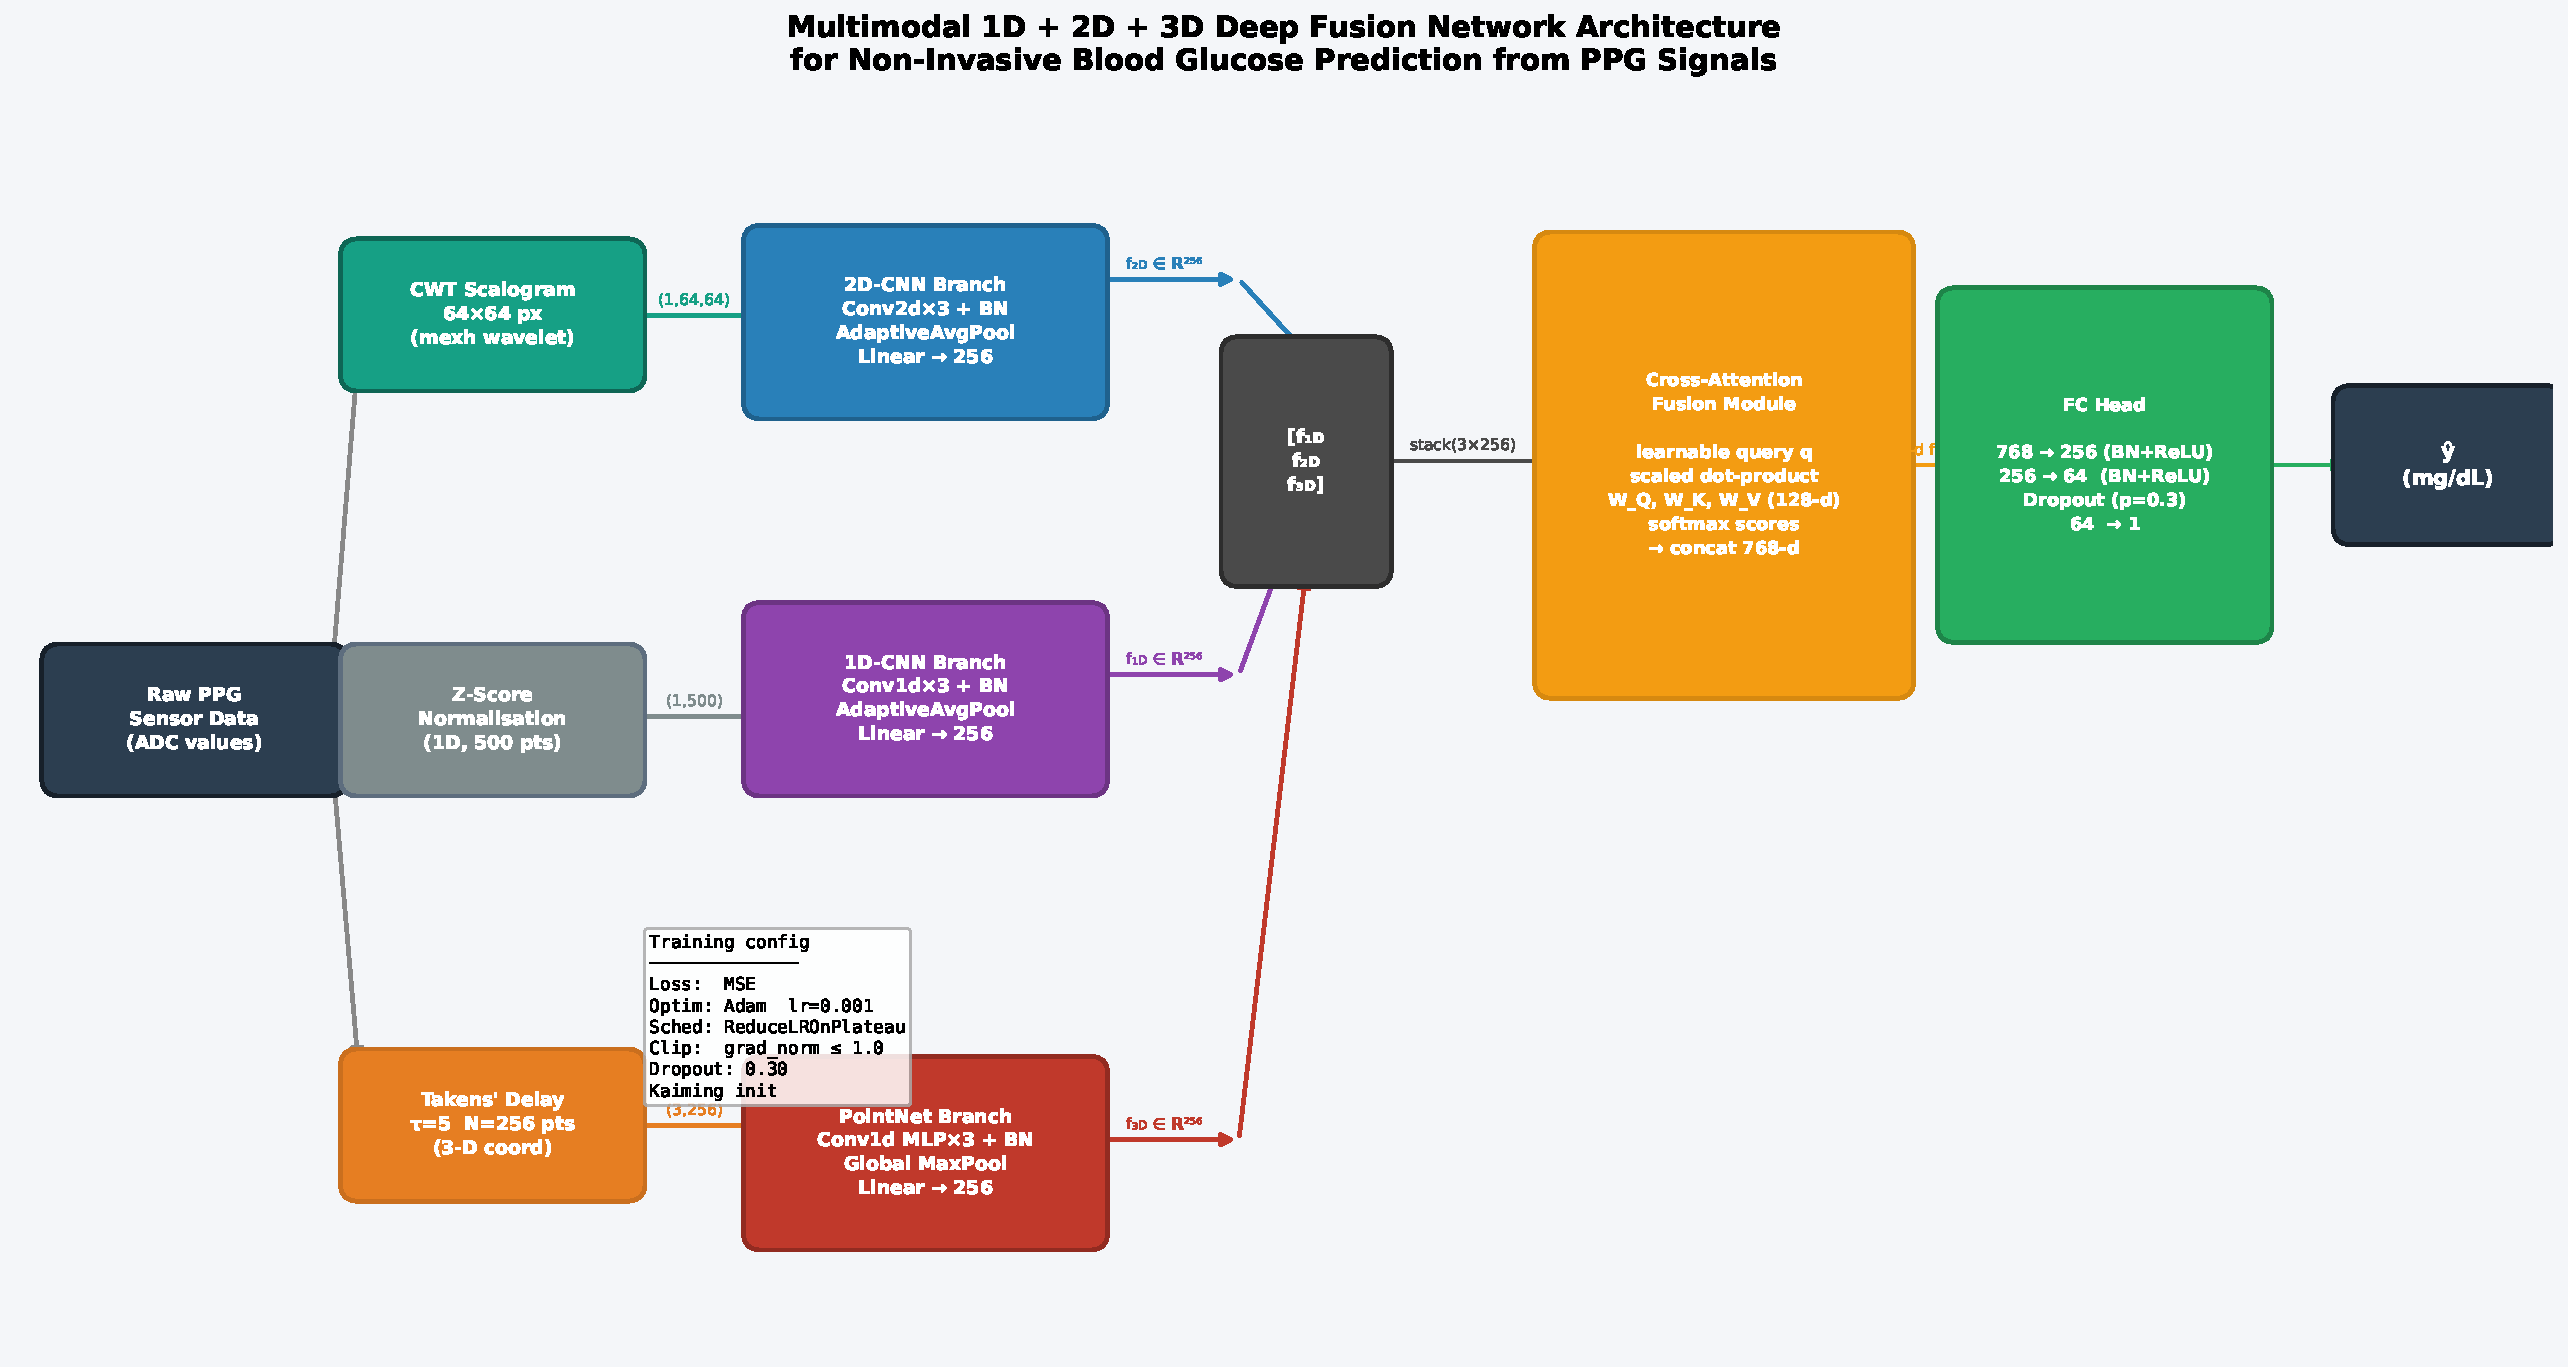
\includegraphics[width=\textwidth]{architecture_diagram.pdf}
  \caption{Proposed Multimodal 1D+2D+3D Fusion Network architecture.
           The raw PPG signal is simultaneously transformed into three
           heterogeneous representations feeding equal-dimension (256-d)
           branch encoders.  A cross-attention module with a learnable
           query vector fuses the branches into a 768-d representation
           passed to the FC regression head.}
  \label{fig:architecture}
\end{figure*}

\begin{figure*}[htbp]
  \centering
  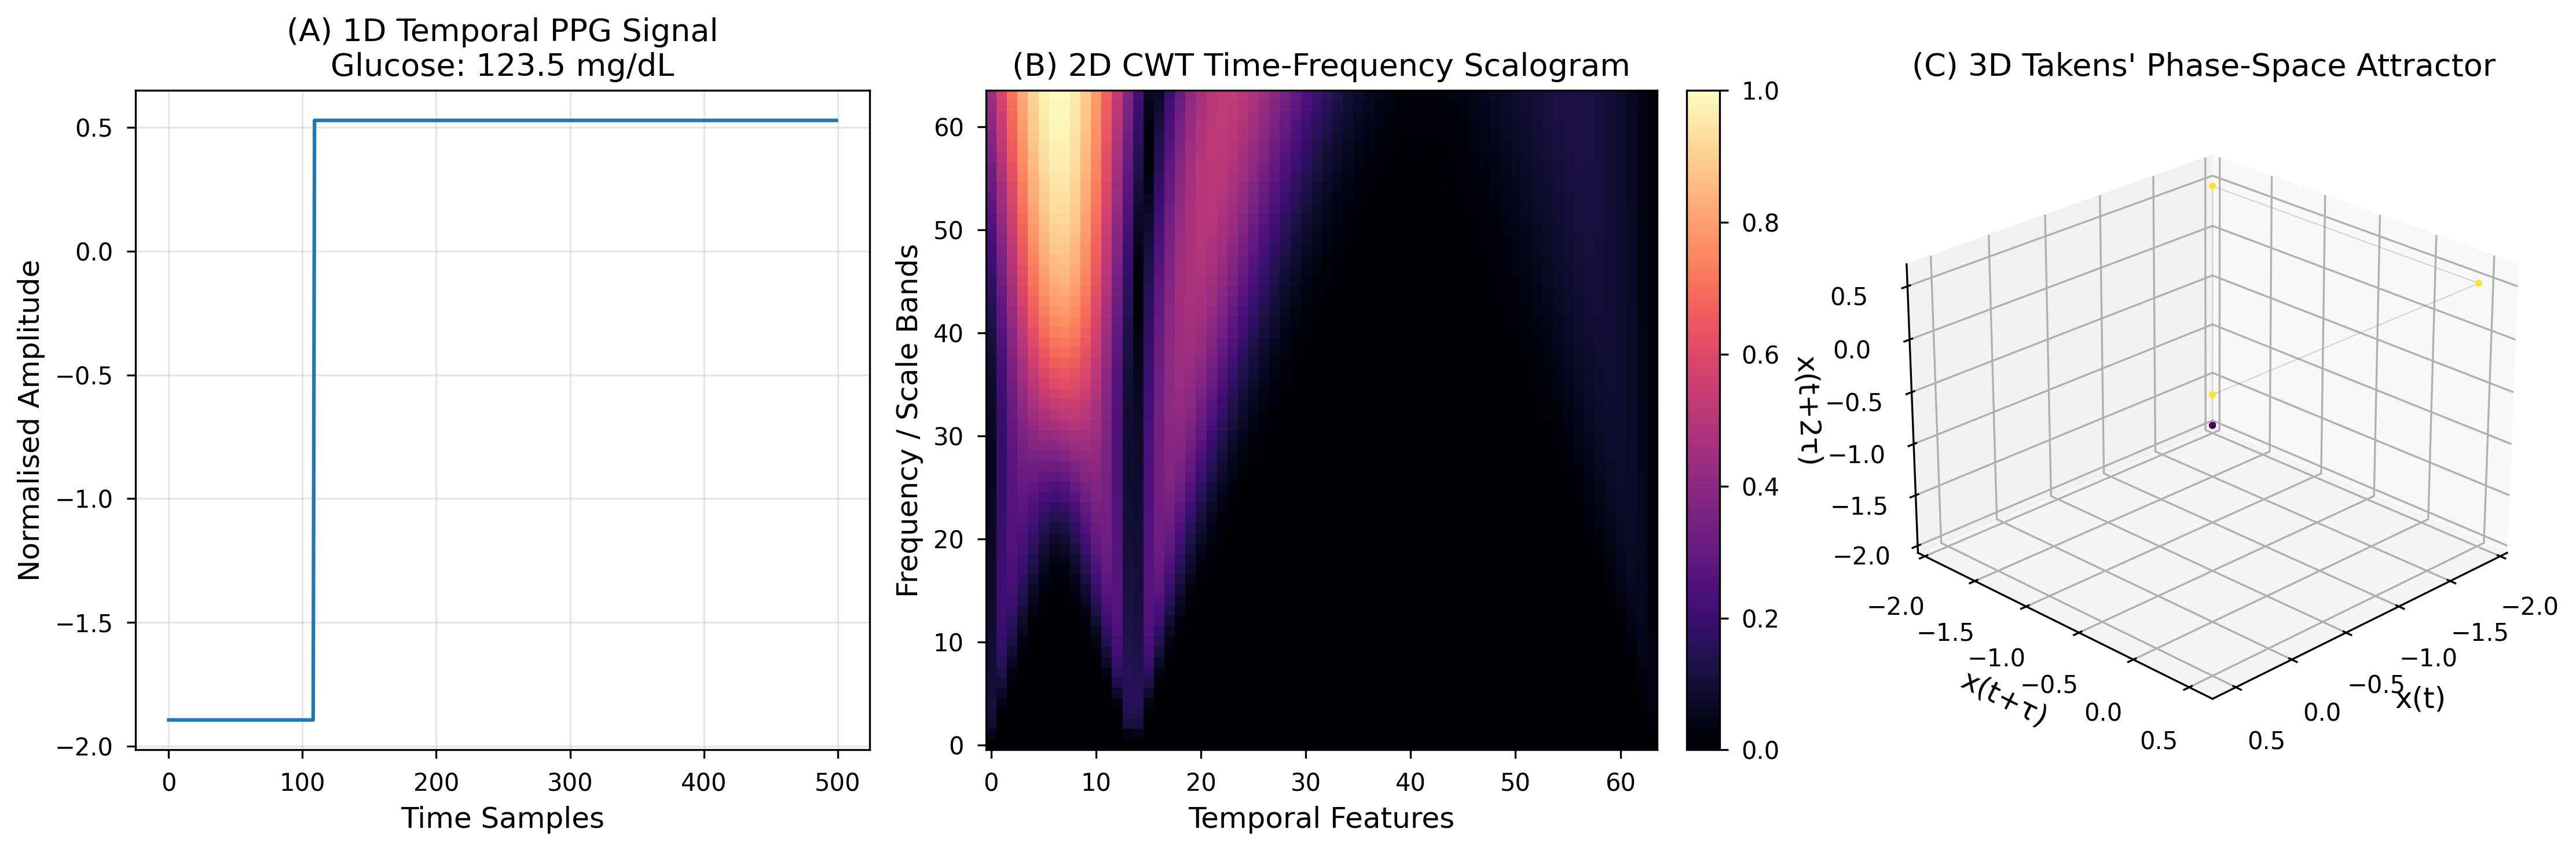
\includegraphics[width=\textwidth]{Paper_Figure_1_Multimodal_Pipeline.png}
  \caption{Example multimodal transformation of a single PPG window
           (sample index 350, glucose $\approx$115~mg/dL).
           \textbf{(A)} Z-score normalised 1D temporal signal;
           \textbf{(B)} 2D CWT time-frequency scalogram ($64\times64$ pixels,
           Mexican hat wavelet);
           \textbf{(C)} 3D Takens delay-embedding phase-space attractor
           ($\tau=5$, $N_p=256$ points), coloured by the third coordinate.}
  \label{fig:pipeline}
\end{figure*}

\begin{figure}[htbp]
  \centering
  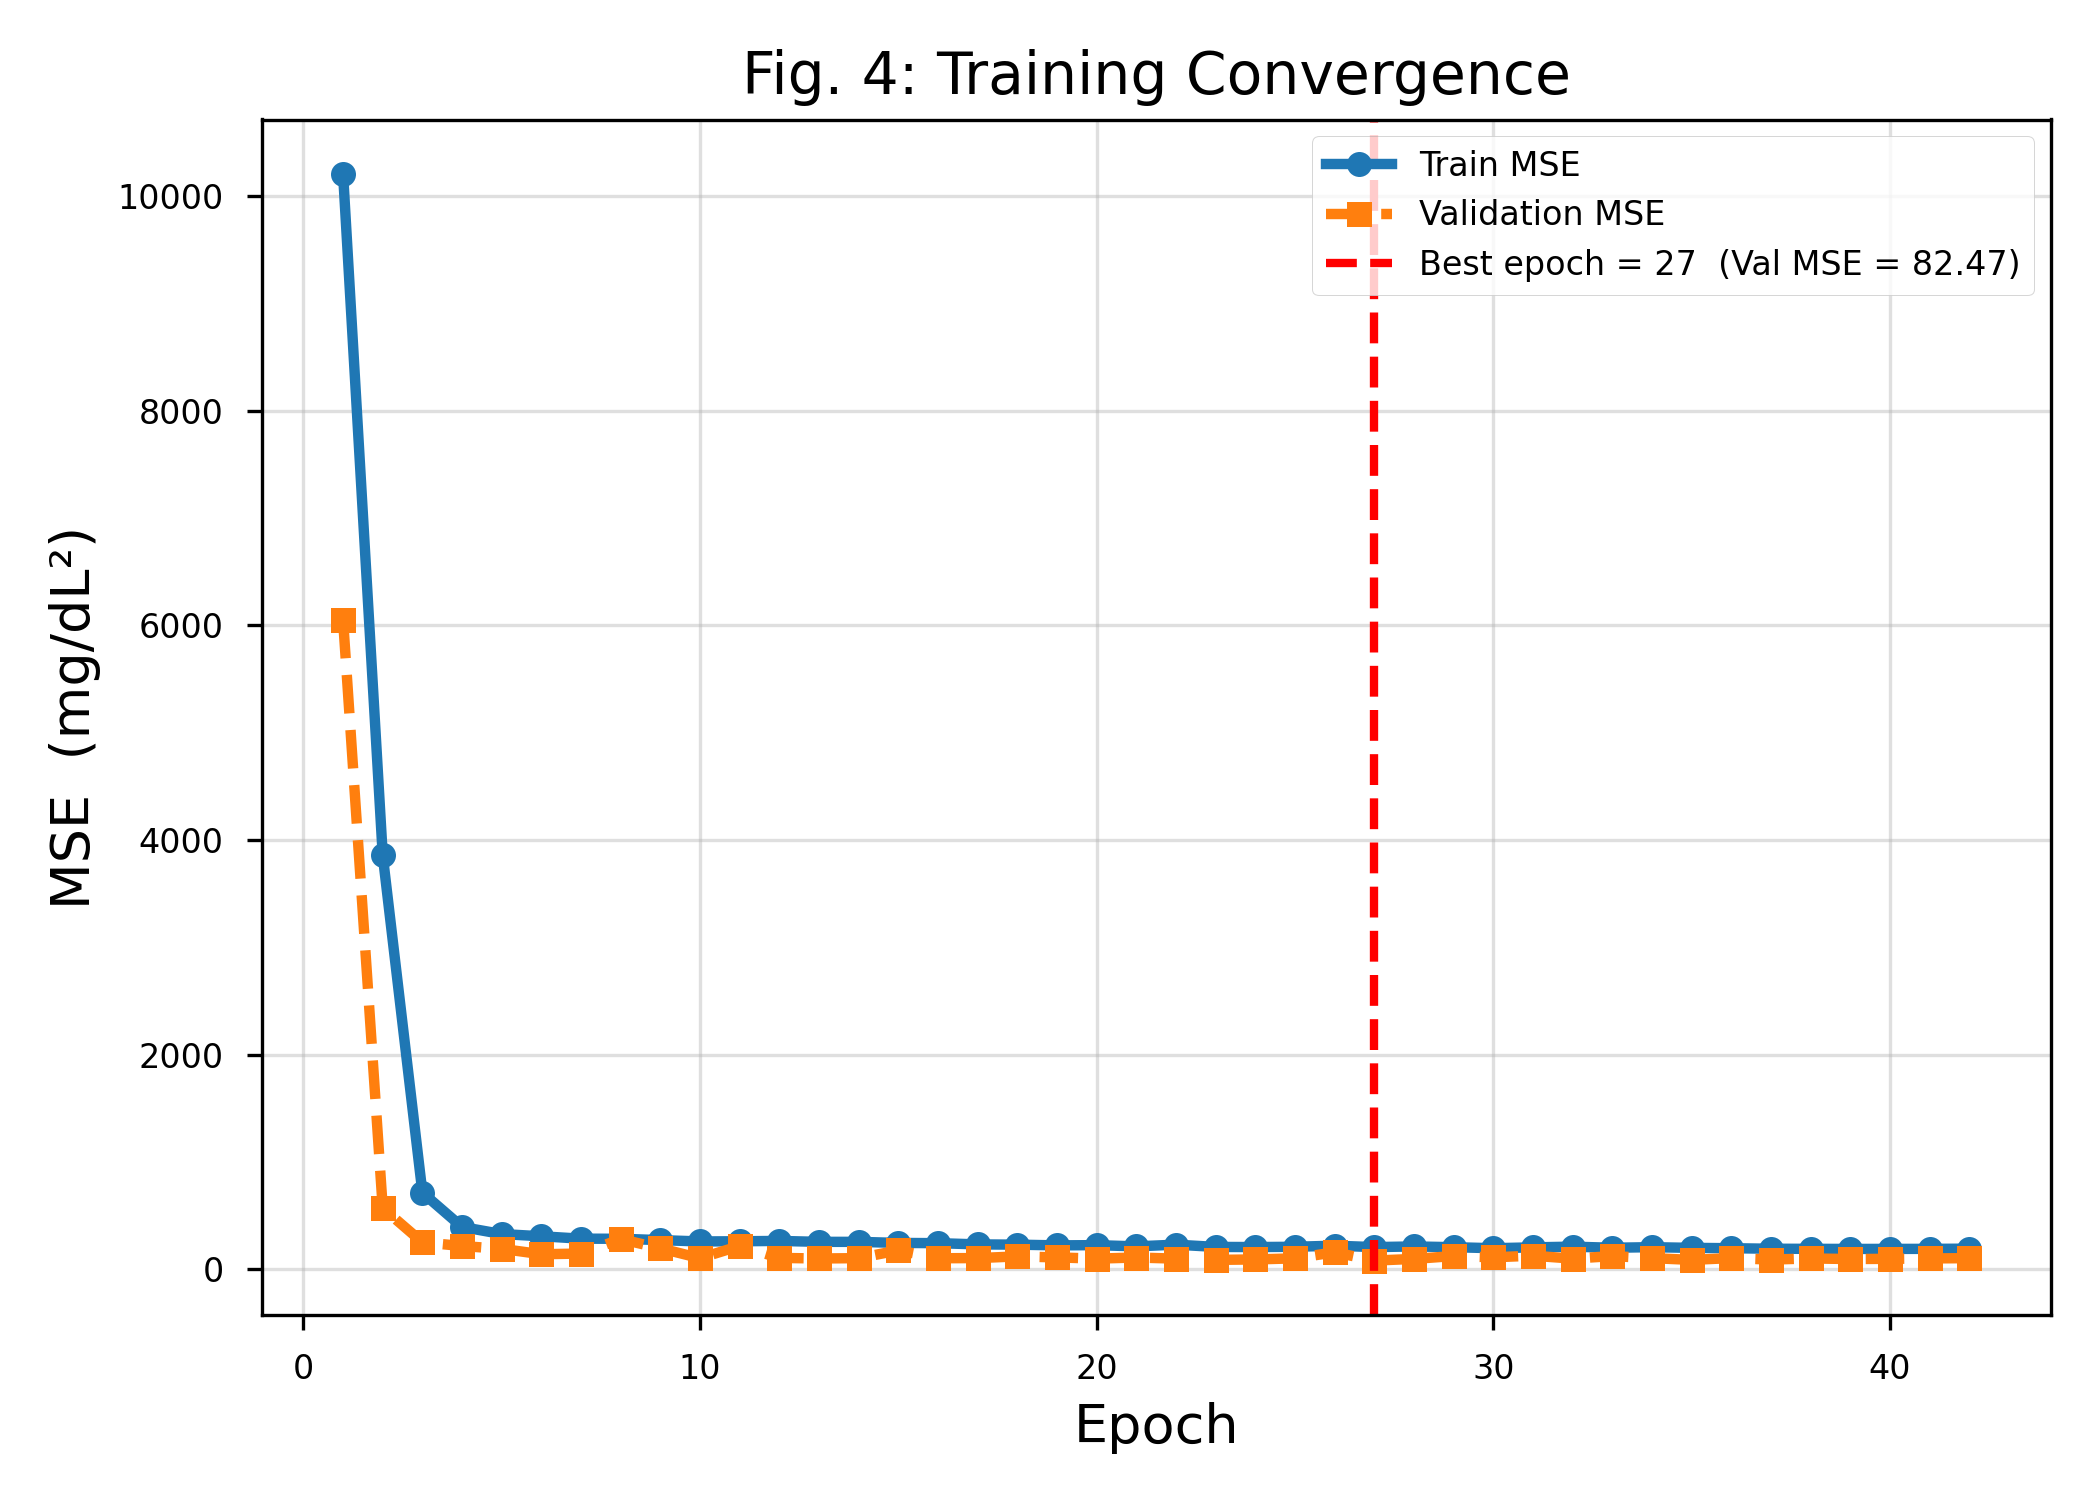
\includegraphics[width=\columnwidth]{Paper_Figure_4_Loss_Curve.png}
  \caption{Training convergence over 42 epochs (early stopped).
           ReduceLROnPlateau halved the LR at epochs 19 and 33
           (vertical arrows not shown).  Best validation MSE of
           82.47~mg/dL² achieved at epoch~27.}
  \label{fig:loss}
\end{figure}

\begin{figure}[htbp]
  \centering
  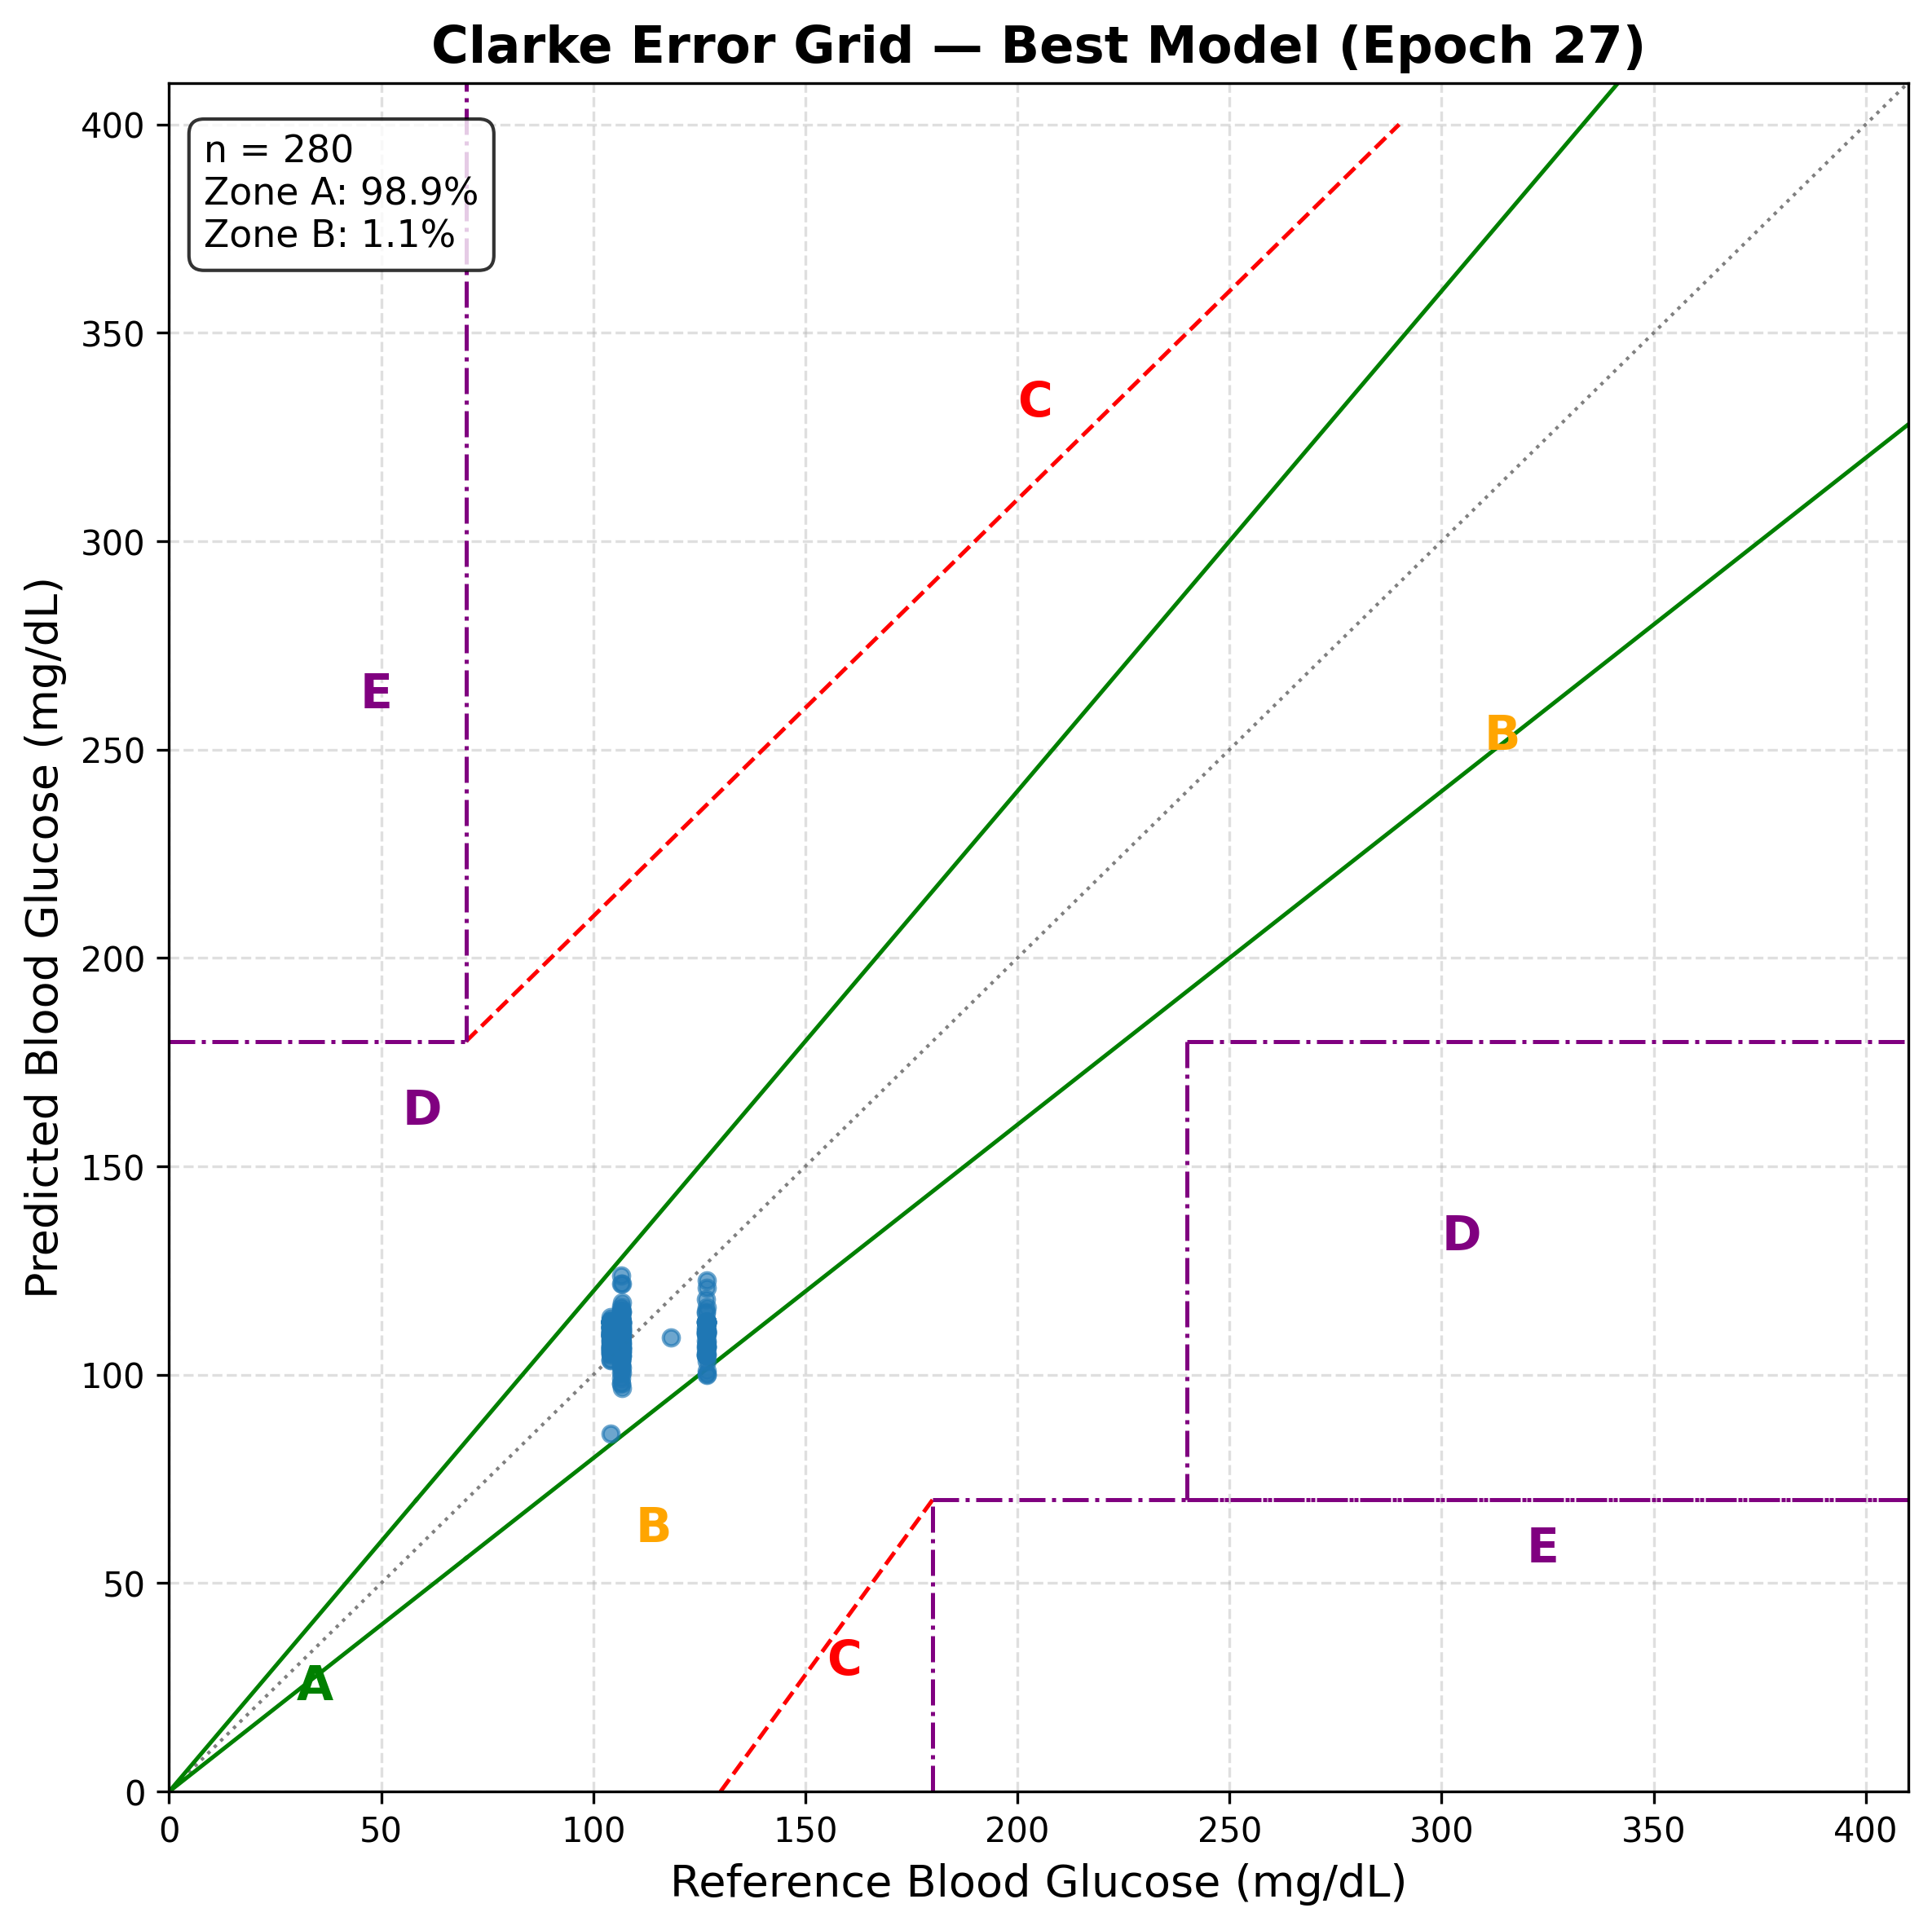
\includegraphics[width=\columnwidth]{clarke_error_grid.png}
  \caption{Clarke Error Grid for 280 validation predictions.
           277 points (98.9\%) lie in Zone~A;
           3 points (1.1\%) lie in Zone~B;
           zero points in Zones C--E,
           indicating strong estimation agreement under the evaluated conditions.}
  \label{fig:clarke}
\end{figure}

\begin{figure}[htbp]
  \centering
  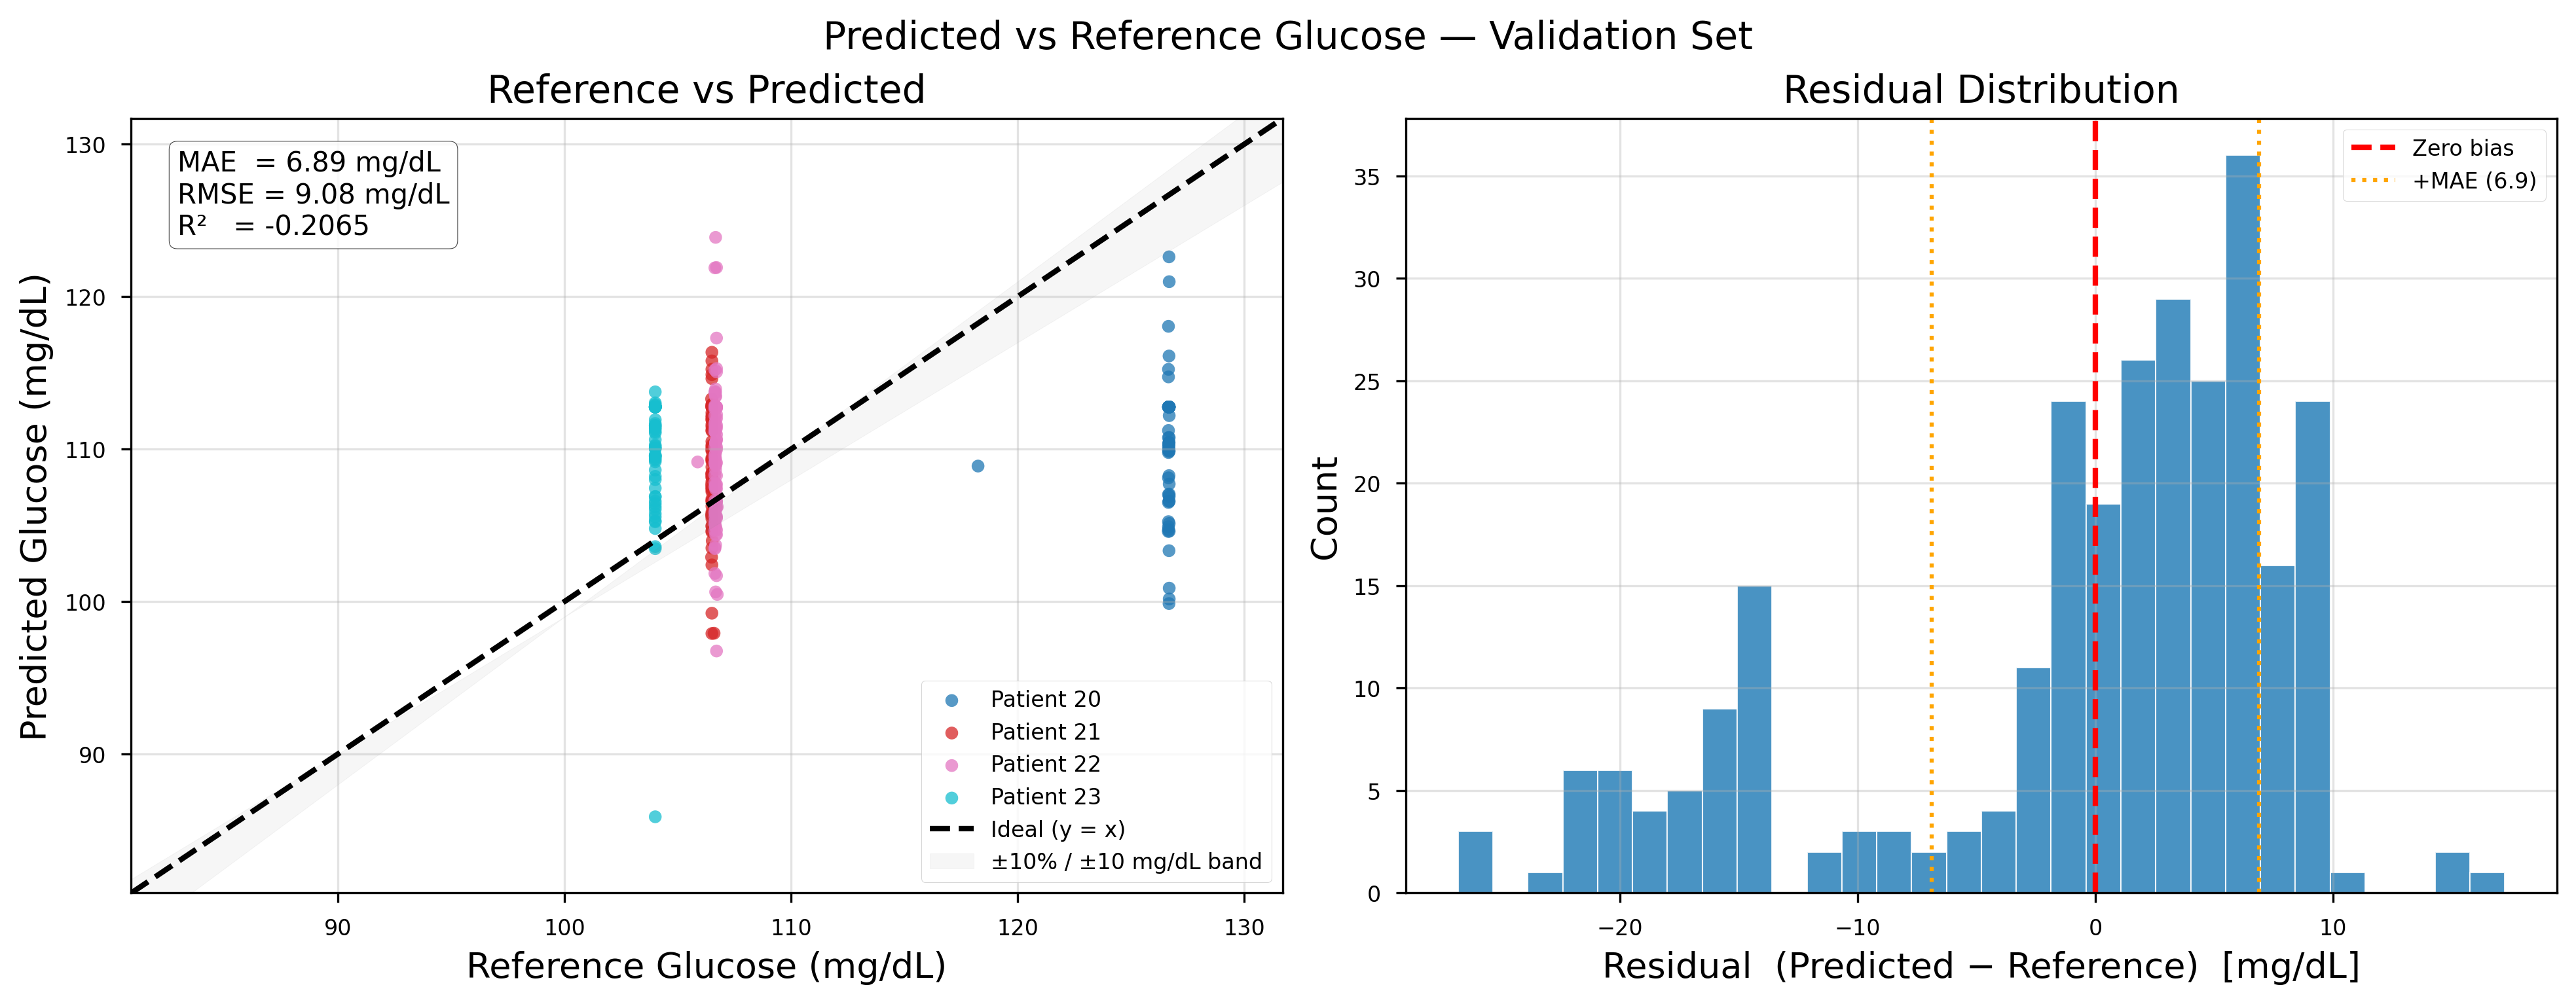
\includegraphics[width=\columnwidth]{overlay_comparison.png}
  \caption{Predicted vs.\ reference glucose scatter (left) and residual
           histogram (right) for the 280-window validation set.
           Points are colour-coded by patient (patients 19--22).
           MAE~=~6.89~mg/dL, RMSE~=~9.08~mg/dL.
           The residual distribution is approximately zero-centred,
           indicating minimal systematic bias.}
  \label{fig:overlay}
\end{figure}

\begin{figure}[htbp]
  \centering
  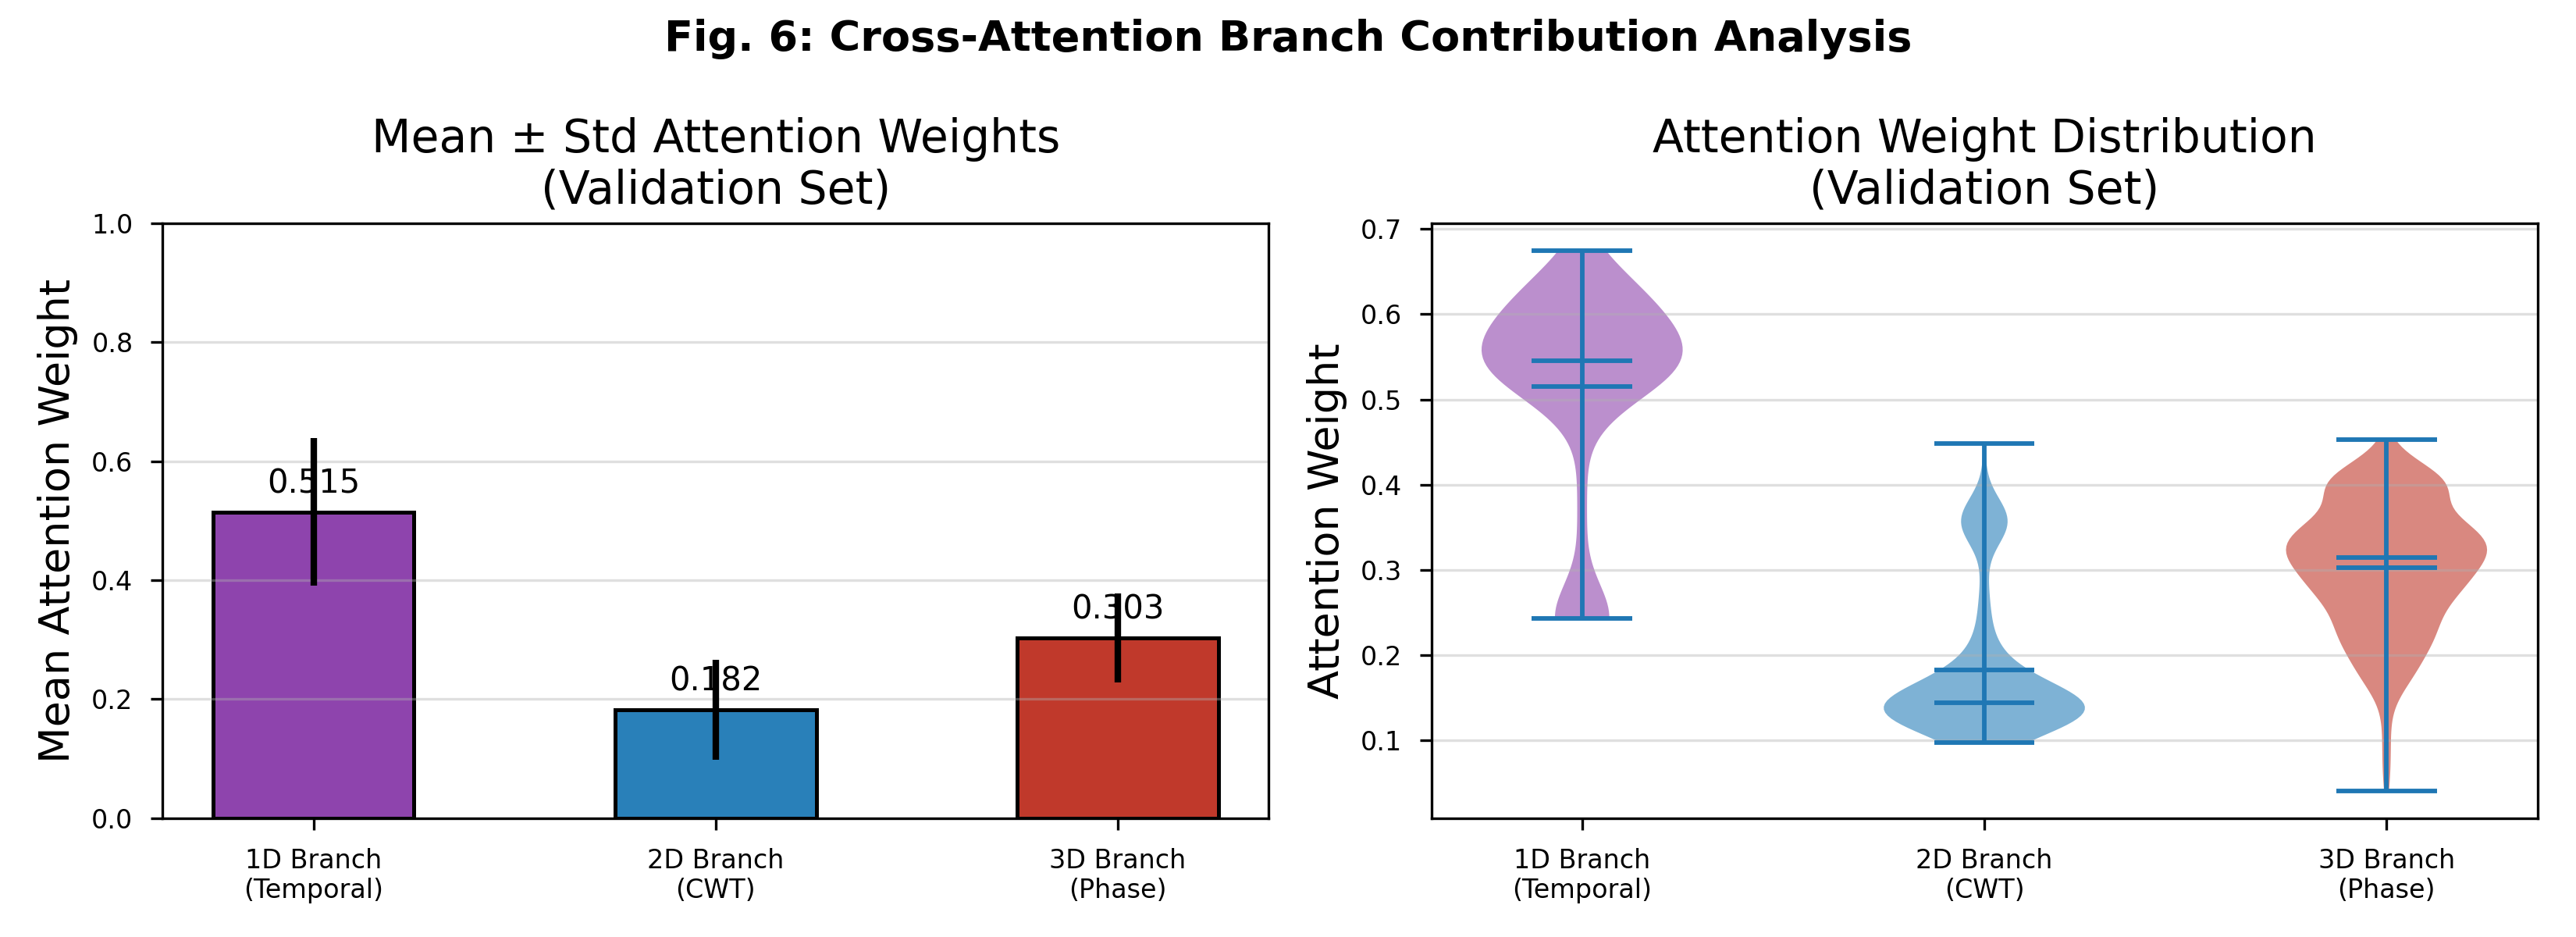
\includegraphics[width=\columnwidth]{Paper_Figure_6_Attention.png}
  \caption{Cross-attention branch weight distribution across 280 validation
           windows.  Left: mean $\pm$ std bar chart; Right: violin plots.
           The 1D temporal branch receives the highest mean weight
           ($0.515\pm0.124$), followed by the 3D phase-space branch
           ($0.303\pm0.075$) and the 2D CWT branch ($0.182\pm0.084$).}
  \label{fig:attention}
\end{figure}

\begin{figure}[htbp]
  \centering
  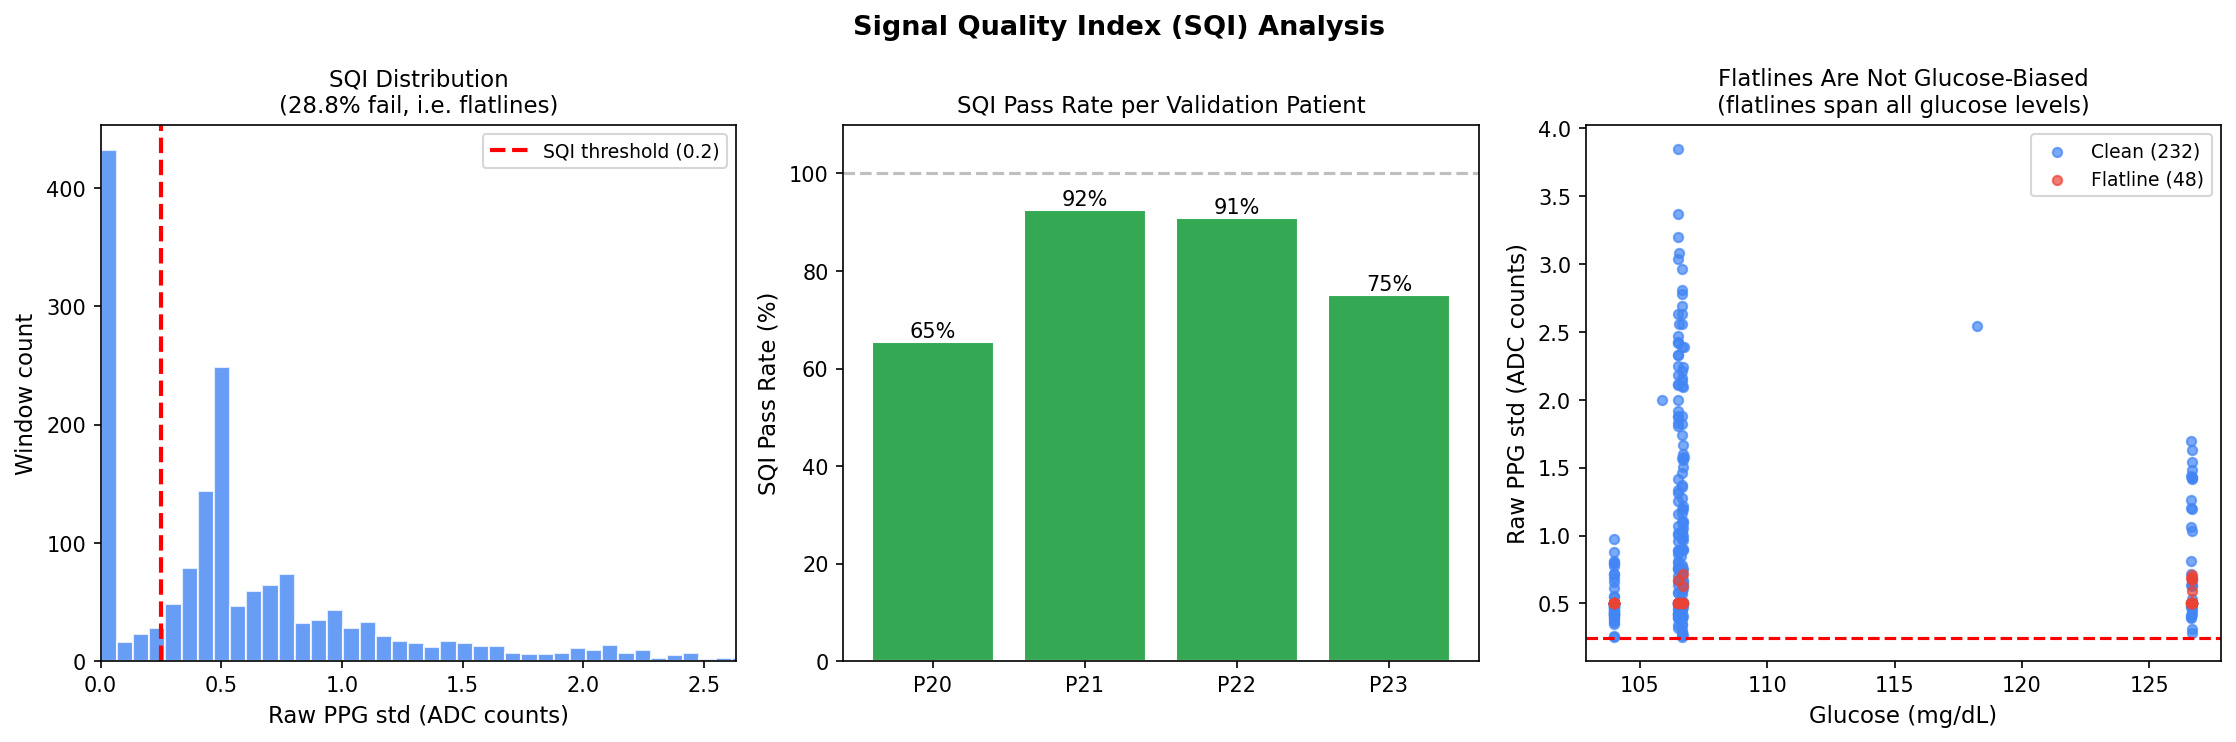
\includegraphics[width=\columnwidth]{Paper_SQI_Analysis.png}
  \caption{Signal Quality Index analysis.  \textbf{Left}: distribution of
           per-window raw PPG standard deviation across all windows
           (threshold $\tau=0.25$, dashed red).
           \textbf{Centre}: per-patient SQI pass rates (patients 19--22).
           \textbf{Right}: SQI vs.\ glucose scatter; flatlines are not
           glucose-biased, confirming artefact-random occurrence.}
  \label{fig:sqi}
\end{figure}

\begin{figure}[htbp]
  \centering
  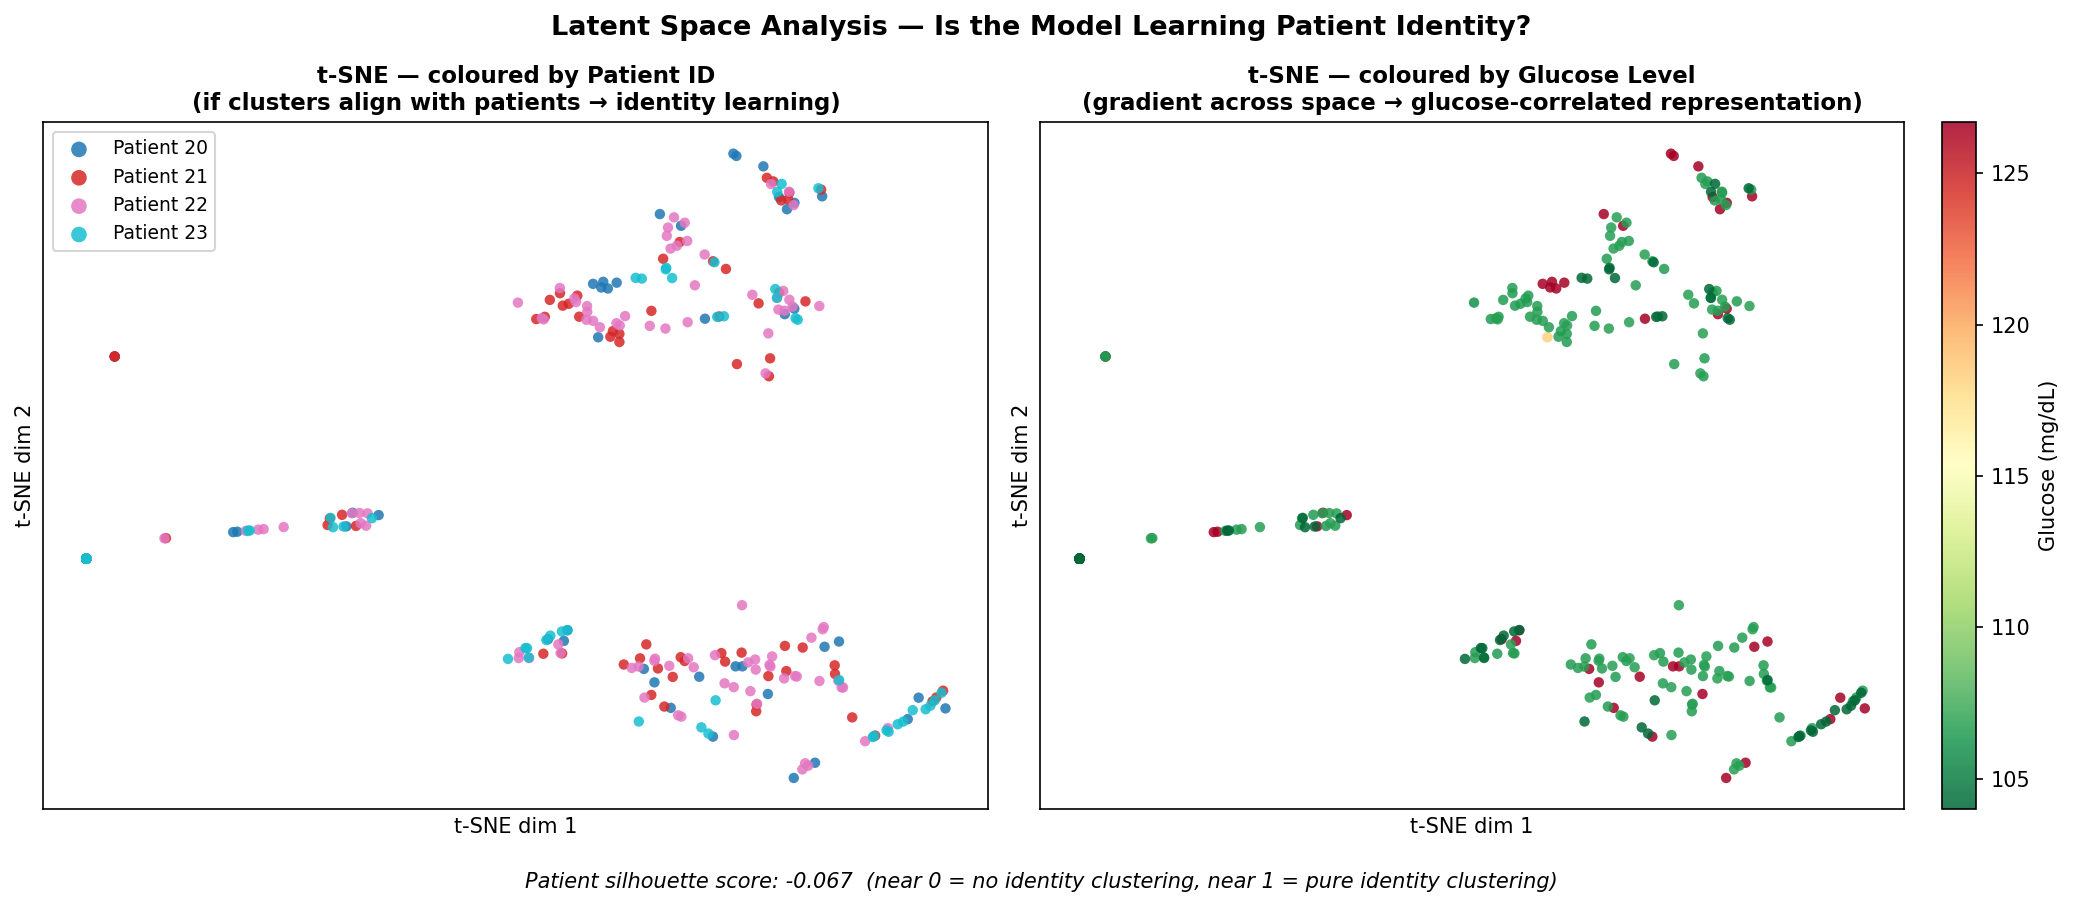
\includegraphics[width=\columnwidth]{Paper_tSNE_Identity.png}
  \caption{t-SNE of the 768-d fused latent space ($n=280$ val windows).
           \textbf{Left}: coloured by patient ID; silhouette score $-0.067$
           confirms no patient-identity clustering.
           \textbf{Right}: coloured by glucose label, showing a diffuse
           glucose gradient rather than sharp identity-driven boundaries.}
  \label{fig:tsne}
\end{figure}

\begin{figure}[htbp]
  \centering
  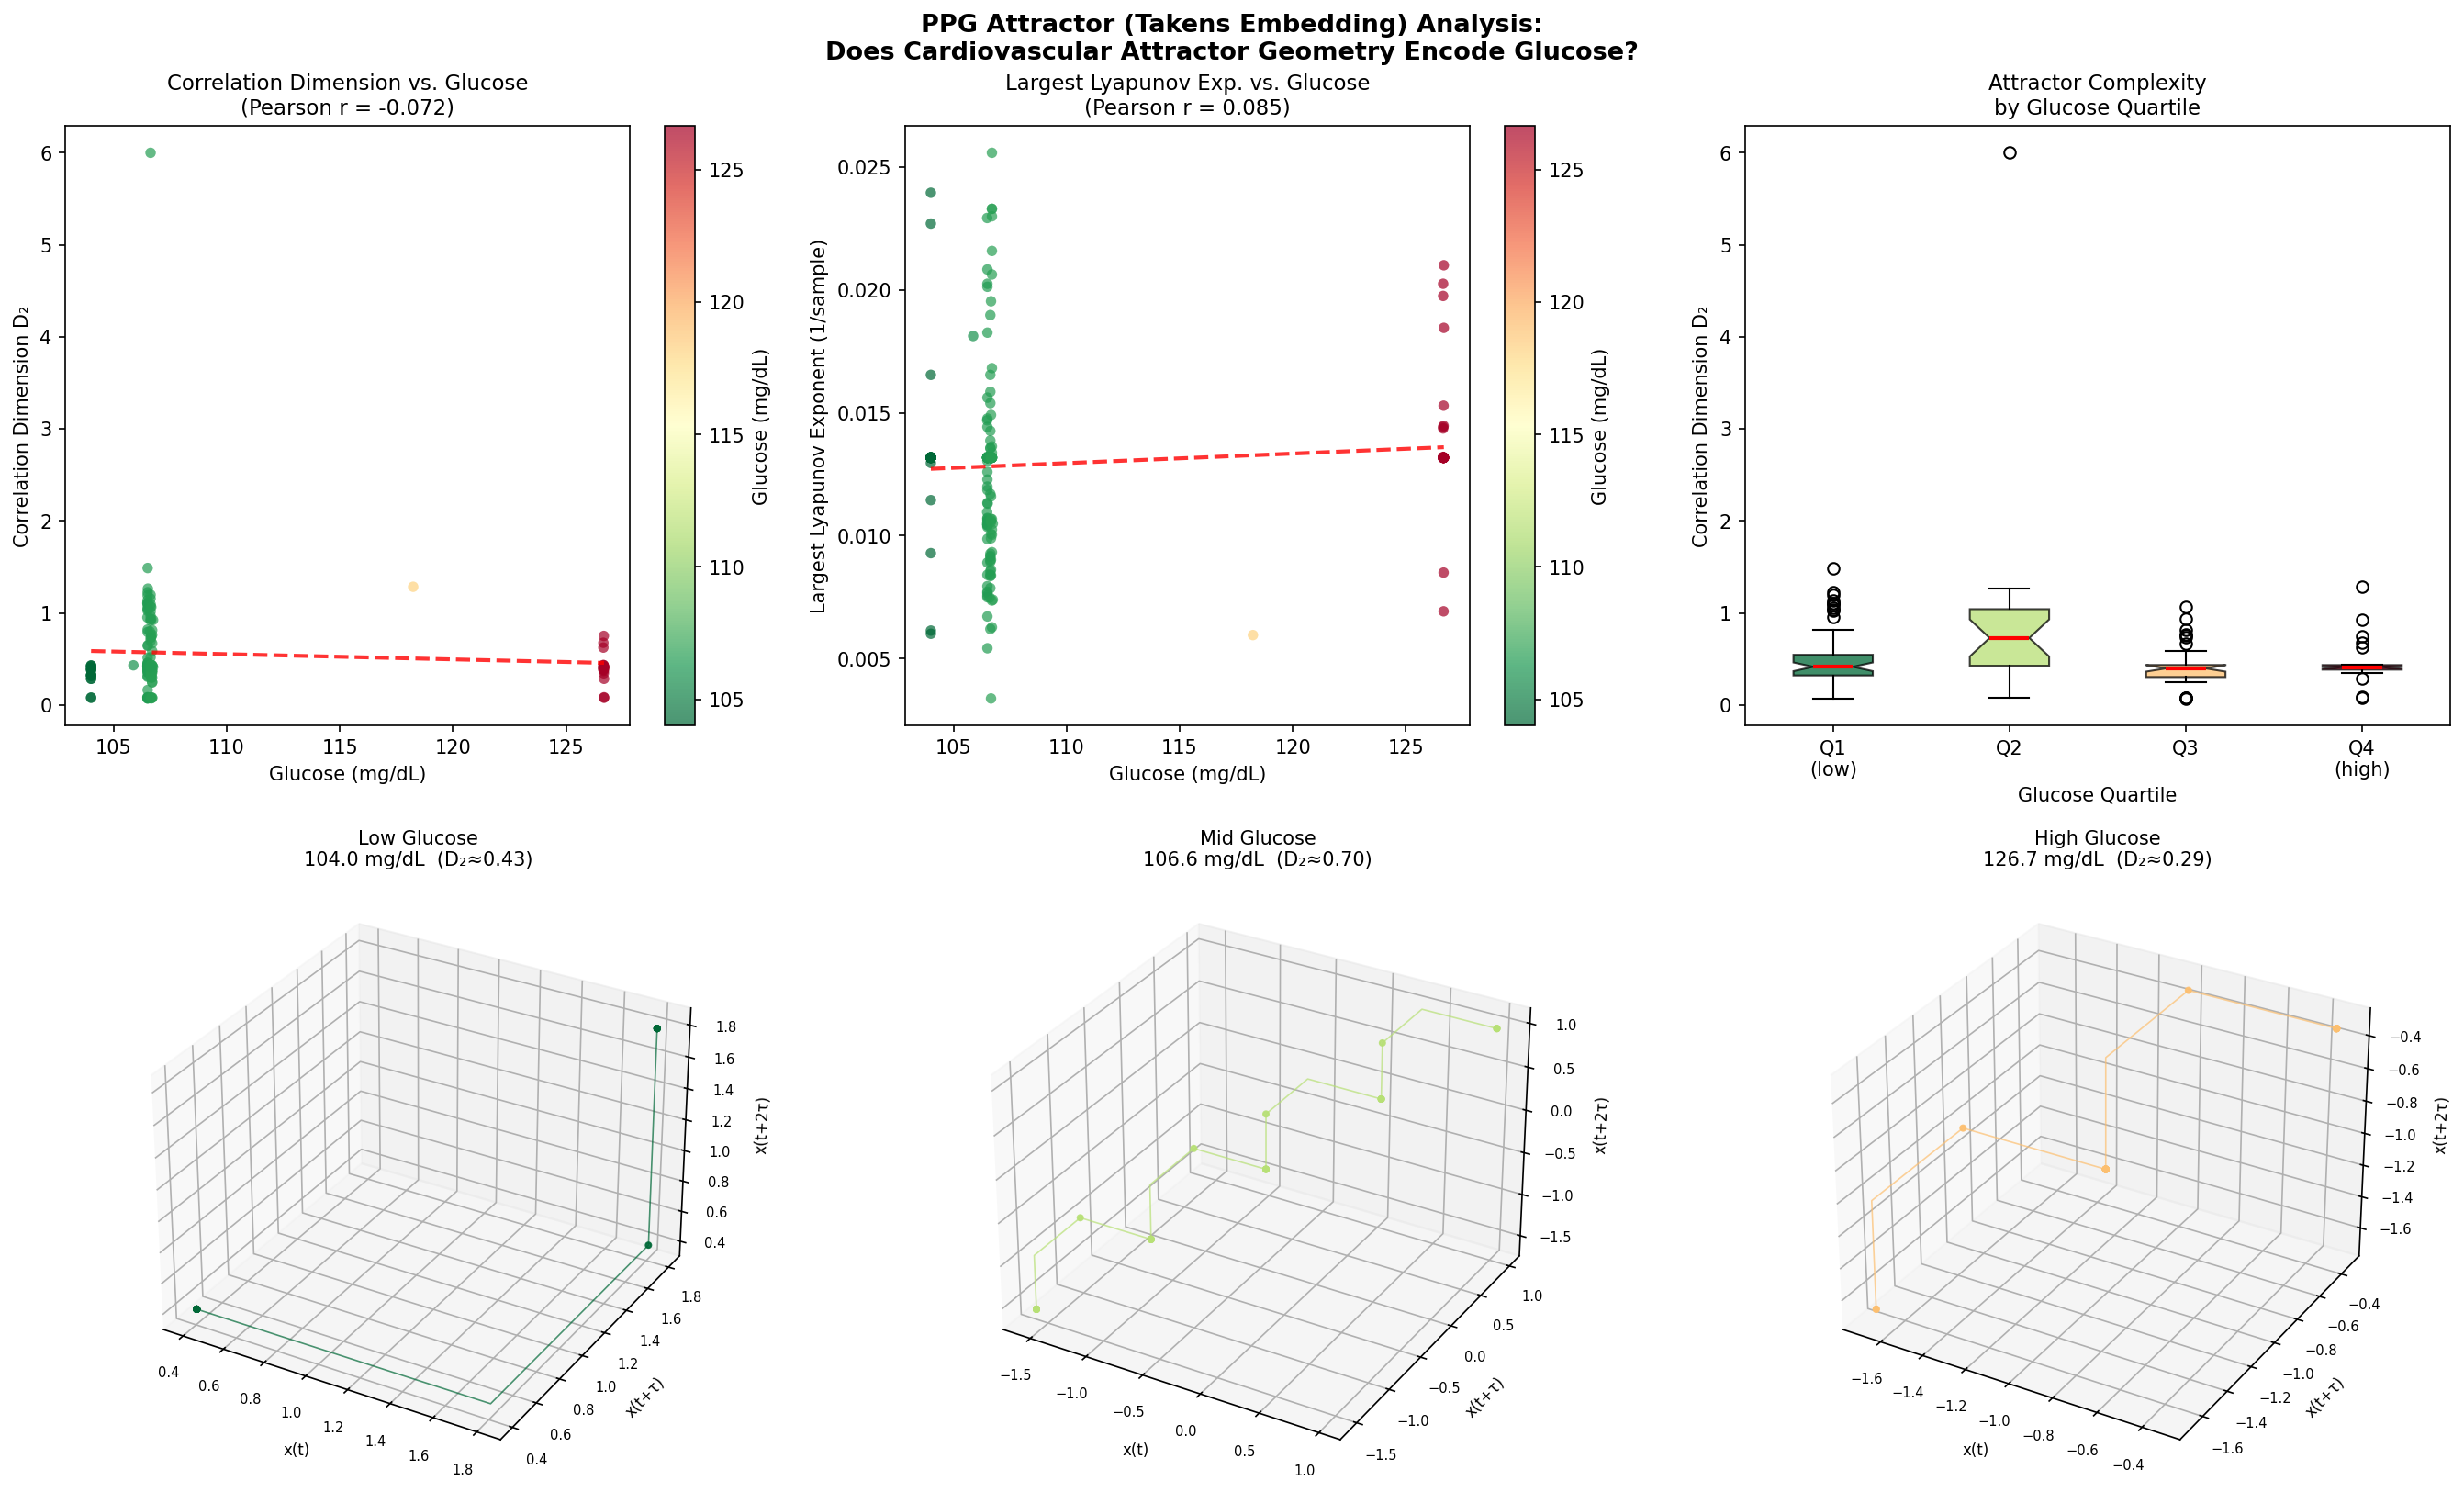
\includegraphics[width=\columnwidth]{Paper_Attractor_Analysis.png}
  \caption{Cardiovascular attractor analysis for SQI-clean validation windows.
           \textbf{Top row}: correlation dimension $D_2$ and largest Lyapunov
           exponent (LLE) versus glucose (Pearson $r=-0.072$ / $r=+0.085$).
           \textbf{Bottom row}: example 3D Takens attractors for low, mid, and
           high glucose windows.}
  \label{fig:attractor}
\end{figure}

\begin{figure}[htbp]
  \centering
  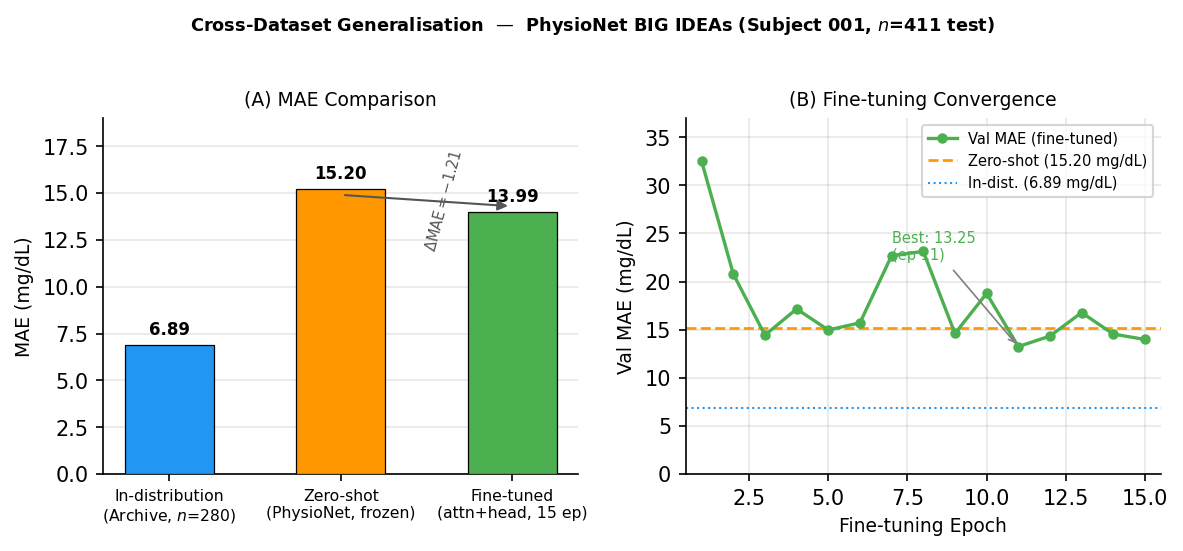
\includegraphics[width=\columnwidth]{Paper_CrossDataset_Generalization.png}
  \caption{Cross-dataset generalisation experiment
           (PhysioNet BIG~IDEAs, Subject~001, Empatica~E4 BVP 64~Hz).
           \textbf{(A)} MAE comparison: in-distribution Archive validation
           (6.89~mg/dL, blue); zero-shot transfer with all weights frozen
           (15.20~mg/dL, orange); fine-tuned cross-attention and head only
           (13.99~mg/dL, green).  The $\Delta$MAE arrow shows $-1.21$~mg/dL
           improvement from fine-tuning.
           \textbf{(B)} Per-epoch validation MAE during 15-epoch fine-tuning
           (Adam, $\eta$=$10^{-3}$, batch~32).  Best val MAE 13.25~mg/dL
           at epoch~11; final reported MAE 13.99~mg/dL at epoch~15.
           Orange dashed: zero-shot baseline (15.20~mg/dL).}
  \label{fig:crossdataset}
\end{figure}

% =============================================================================
% References
% =============================================================================
\begin{thebibliography}{99}

\bibitem{idf2021}
International Diabetes Federation,
``IDF Diabetes Atlas, 10th Edition,''
Brussels, Belgium: IDF, 2021.
[Online]. Available: \url{https://diabetesatlas.org}

\bibitem{allen2007ppg}
J.~Allen,
``Photoplethysmography and its application in clinical physiological
measurement,''
\textit{Physiological Measurement}, vol.~28, no.~3, pp.~R1--R39, 2007.

\bibitem{hina2021noninvasive}
A.~Hina and M.~R.~Mahfouz,
``Noninvasive blood glucose monitoring systems using near-infrared technology
--- a review,''
\textit{Sensors}, vol.~22, no.~1, p.~icz, 2022.

\bibitem{dinh2022ppg}
T.-L.-A.~Dinh, N.-T.~Nguyen, B.-L.~Nguyen, and V.-T.~Tran,
``Non-invasive blood glucose estimation using photoplethysmography and
deep learning,''
in \textit{Proc.\ IEEE Int.\ Conf.\ Biomed.\ Eng.\ (ICBME)}, 2022.

\bibitem{almarshad2021}
M.~A.~Almarshad, M.~S.~Islam, S.~Al-Ahmadi, and A.~S.~BaHammam,
``Diagnostic features and potential applications of PPG signal in healthcare:
a systematic review,''
\textit{Healthcare}, vol.~10, no.~3, p.~547, 2022.

\bibitem{takens1981}
F.~Takens,
``Detecting strange attractors in turbulence,''
in \textit{Dynamical Systems and Turbulence, Lecture Notes in Mathematics},
D.~Rand and L.-S.~Young, Eds.
Berlin: Springer, 1981, vol.~898, pp.~366--381.

\bibitem{qi2017pointnet}
C.~R.~Qi, H.~Su, K.~Mo, and L.~J.~Guibas,
``PointNet: Deep learning on point sets for 3D classification and segmentation,''
in \textit{Proc.\ IEEE Conf.\ Comput.\ Vision Pattern Recognit.\ (CVPR)},
Honolulu, HI, USA, 2017, pp.~652--660.

\bibitem{vaswani2017attention}
A.~Vaswani, N.~Shazeer, N.~Parmar, J.~Uszkoreit, L.~Jones, A.~N.~Gomez,
{\L}.~Kaiser, and I.~Polosukhin,
``Attention is all you need,''
in \textit{Proc.\ Adv.\ Neural Inf.\ Process.\ Syst.\ (NeurIPS)},
Long Beach, CA, USA, 2017, pp.~5998--6008.

\bibitem{he2015init}
K.~He, X.~Zhang, S.~Ren, and J.~Sun,
``Delving deep into rectifiers: Surpassing human-level performance on
ImageNet classification,''
in \textit{Proc.\ IEEE Int.\ Conf.\ Comput.\ Vision (ICCV)},
Santiago, Chile, 2015, pp.~1026--1034.

\bibitem{li2020ecg}
X.~Li, X.~Qian, L.~Zhu, X.~Kong, Z.~Wen, and J.~Li,
``Automatic staging of sleep disorders using a multi-scale CNN-LSTM
architecture,''
\textit{IEEE Trans.\ Neural Syst.\ Rehabil.\ Eng.}, vol.~28,
no.~10, pp.~2245--2254, 2020.

\bibitem{clarke1987}
W.~L.~Clarke, D.~Cox, L.~A.~Gonder-Frederick, W.~Carter,
and S.~L.~Pohl,
``Evaluating clinical accuracy of systems for self-monitoring of blood glucose,''
\textit{Diabetes Care}, vol.~10, no.~5, pp.~622--628, 1987.

\bibitem{ppgdataset2023}
``PPG Glucose Dataset,''
Kaggle, 2023.
[Online]. Available: \url{https://www.kaggle.com/}

\bibitem{vandermaaten2008tsne}
L.~J.~P.~van der Maaten and G.~E.~Hinton,
``Visualizing high-dimensional data using t-SNE,''
\textit{J.\ Machine Learning Research}, vol.~9, pp.~2579--2605, 2008.

\bibitem{bigideas2023}
BIG IDEAs Lab,
``BIG IDEAs Lab Glycemic Variability \& Wearable Device Dataset,"
\textit{PhysioNet}, v1.1.3, 2023.
[Online]. Available: \url{https://doi.org/10.13026/aw6y-fc44}

\end{thebibliography}

\end{document}
